\documentclass[11pt,letterpaper]{article}
%\usepackage[labelformat=bf]{caption}
\usepackage[graphicx]{realboxes}
\setcounter{topnumber}{3}% Just for this example
\usepackage[font={footnotesize,it}]{caption}
\usepackage{amsmath,amssymb,url,appendix,anysize,fancyhdr,float,epstopdf}
\usepackage[utf8]{inputenc}
\usepackage[spanish,mexico]{babel}
\usepackage{helvet}
\usepackage{caption}
\captionsetup{font=footnotesize}
\renewcommand{\familydefault}{\sfdefault}
%\renewcommand*{\bibfont}{\footnotesize}
%\renewcommand{\bibsection}{}
\graphicspath{{./Img/},{./Portada/}}
\DeclareGraphicsExtensions{.jpeg,.bmp,.png,.jpg,.eps,.pdf}
\renewcommand{\appendixname}{Apéndices}
\renewcommand{\appendixtocname}{Apéndices}
\renewcommand{\appendixpagename}{Apéndices}
\renewcommand{\rmdefault}{ptm}
%\renewcommand\Authfont{\fontsize{20}{14.4}\selectfont}
%\numberwithin{figure}{subsection}
\numberwithin{equation}{subsection}
\numberwithin{table}{subsection}
\usepackage[colorlinks=true,linkcolor=black,urlcolor=black,citecolor=black]{hyperref}
\marginsize{2cm}{2.5cm}{2.5cm}{2.5cm}
\pagestyle{fancy}
\lhead{CIC}
\chead{\rightmark}
\rhead{Tesina}
\lfoot{.}
\cfoot{\thepage}
\rfoot{.}
\renewcommand{\headrulewidth}{0.4pt}
\renewcommand{\footrulewidth}{0.4pt}
\usepackage{amsmath,amssymb,amsthm,amscd}
\usepackage{amssymb, amsmath, amsbsy} % librerias ams
\usepackage{upgreek} % para poner letras griegas sin cursiva
\usepackage{mathdots} % para el comando \iddots
\usepackage{longtable}
\renewcommand{\baselinestretch}{1.25}
\usepackage{hyperref}
\hypersetup{
    colorlinks=true,
    linkcolor=black,
    filecolor=magenta,      
    urlcolor=blue,
    pdftitle={Overleaf Example},
    pdfpagemode=FullScreen,
    }


\begin{document}
\begin{titlepage}

\begin{center}
\newcommand{\HRule}{\rule{\linewidth}{0.5mm}}


%\includegraphics[width=0.95\textwidth]{Portada/Logo.png}\vspace*{1cm}

\textsc{\LARGE Instituto Politécnico Nacional}\\[0.5cm]
\textsc{\LARGE Centro de Investigación en Computación }\\[1.5cm]

% ------------------------------------- EDIT -------------------------------------
\textsc{\Large Doctorado en ciencias de la computación }\\[0.5cm]
\textsc{\Large }\\[0.5cm]

\HRule \\[0.4cm]
{ \huge \bfseries Decodificación neuronal mediante Redes Neuronales Profundas}\\[0.1cm]
\HRule \\[1cm]


\begin{minipage}{0.8\textwidth}
\begin{center} \large
\textbf{PRESENTA}\\
Santiago Isaac Flores Alonso\\
	
	

\end{center}
%\vspace*{0.5 cm}
\end{minipage}
%\vspace*{0.5 cm}
%\begin{minipage}{0.8\textwidth}
%\begin{flushright} \large
%M. En C. Ricardo Roberto Horta Olivares\\
%Profesor
%\end{flushright}
%\end{minipage}

%\vfill
\bigskip
\large \textbf{DIRIGE:}\\
{\large} Dr. René Luna García
\end{center}

\end{titlepage}

\newpage
\tableofcontents
\vfill

\newpage
\renewcommand{\abstractname}{Decodificación neuronal mediante Redes Neuronales Profundas}
%\thispagestyle{empty}

%\begin{abstract}

%\noindent La presente propuesta se centra en el uso de técnicas de aprendizaje automático, métodos computacionales y registros EEG, con el objetivo de desarrollar un modelo capaz de predecir la evolución al síndrome de Lennox-Gastaut en pacientes diagnosticados con síndrome de West, proporcionando un enfoque novedoso en la implementación de la inteligencia artificial como un mecanismo viable para prevenir y tratar la epilepsia refractaria en las etapas previas a su desarrollo.

\section{Introducción }

\noindent El sistema nervioso central es una estructura bilateral y esencialmente simétrica con siete partes fundamentales: médula espinal, bulbo raquídeo, protuberancia, cerebelo, mesencéfalo, diencéfalo y hemisferios cerebrales. Las operaciones cerebrales responsables de nuestras capacidades cognitivas (atención, memoria, percepción, lenguaje, planeación motora, etc.) ocurren fundamentalmente en la corteza cerebral: un tejido de coloración gris que recubre los hemisferios \cite{Kandel2000}, el cual tiene una organización conocida como \textit{procesamiento paralelo distribuido}, o en palabras de Donald Hebb se entiende que $"$la capacidad del cerebro se deriva de la orquestación espacio-temporal de la actividad neuronal$"$ \cite{Hebb2005}. 

\bigskip
\noindent Al día de hoy, gracias a los esfuerzos de múltiples áreas del conocimiento como la psicología, medicina, neurobiolgía, biología molecular, ingeniería, física y química, se antoja apropiado comparar al cerebro con una compleja computadora naturalmente evolucionada, constituidas orgánicamente, analógicas en representación y paralela en su arquitectura de procesamiento, que en el caso de los seres humanos, confiere la capacidad de incluso reflexionar sobre nuestra (su) propia existencia \cite{Churchland1994}. Sin embargo, existe una gran diferencia entre los sistemas biológicos y los digitales: los sistemas biológicos son plásticos. Esta capacidad implica la reorganización estructural y funcional de las conexiones inter e intra regiones cerebrales \cite{costandi2016neuroplasticity}, a diferencia de los sistemas digitales que son inherentemente estáticos. Esta capacidad, mediada por factores genéticos y ambientales, nos permite adaptarnos, aprender y con el tiempo, define nuestra individualidad.

\bigskip
\noindent El macroefecto mostrado por el sistema nervioso, es producto de la interacción de 15 mil millones de elementos unitarios de procesamiento, las neuronas, las cuales forman parte de sistemas locales especializados identificables por su función, agrupadas en un órgano de apenas 1500 gramos \cite{Kandel2000}. El paradigma de estructuras anatómicas que constituye a las neuronas incluye tanto a los axones para enviar señales, como proliferaciones arbóreas (dendritas) para recibir señales y un núcleo de integración (soma); estas células son esencialmente dispositivos eléctricos y su actividad básica es recibir y transmitir señales provocando y respondiendo a la corriente eléctrica. Cada neurona recibe información, en promedio, a través de unas 10 mil sinapsis y envía información a través de otras mil, formando un complejo sistema con innumerables puntos de comunicación. %que dan forma a fenómenos como la conciencia, imaginación, memoria, movimiento, etc. (faltan citas.)


\bigskip
\noindent Explicar como estos estos fenómenos convergen y se traduce en conductas complejas, es una de las grandes fronteras de la ciencia actual. Ciertamente, resulta fascinante considerar que cuando hablamos de comprender el funcionamiento cerebral, estamos aludiendo a los esfuerzos de un órgano para conocerse a sí mismo, pero $"$¿Podrá el producto, la mente, comprender al aparato productor?$"$ \cite{arechiga2014universo}. En las últimas tres décadas, se ha aprendido mucho sobre el cerebro: sobre su electrofisiología, microanatomía, conectividad y desarrollo; sobre la neurona, su membrana, los tipos de canales y sus funciones específicas en la recepción, integración y envío de señales; sobre la liberación del transmisor y como median la señalización de una neurona a la siguiente, sobre el rango, la estructura y los mecanismos de los receptores \cite{Levitan1991, Chappell2020}. Incluso, hoy en día se descubren nuevos receptores, y la genética de las proteínas que los constituyen y su estructura tridimensional sigue siendo un gran campo de investigación.

\bigskip
\noindent Pero, si sabemos tanto sobre neuronas ¿por qué no comprendemos todavía cómo funciona el cerebro? y sobre todo ¿qué nos hace individuos? El argumento general es que el conocimiento de los niveles molecular y celular es esencial, pero por sí solos no son suficiente, por más rico y completo que sea. Los comportamientos complejos son el resultado de la dinámica de las redes neuronales. Esto significa que, si bien las propiedades de la red dependen de las propiedades de las neuronas en la red, no son idénticas a las propiedades celulares ni a combinaciones simples de propiedades celulares \cite{Bailek1991} y aunque usualmente entendemos al sistema nervioso como una sola entidad, en realidad parece ser una colección interconectada de sistemas de propósito especial que son muy eficientes en la realización de sus tareas, pero con una flexibilidad limitada \cite{Churchland1994}. Por lo que, aunque se entienda el funcionamiento micro-estructural y la organización macro-estructural del cerebro, es a nivel meso-estructural, al nivel de las interacción entre regiones donde encontraremos el substrato neuronal que pueda explicar el comportamiento.  

\bigskip
\noindent En este punto es importante definir 


\bigskip
\noindent En este contexto, surge la interrogante de si es factible identificar características estructurales y funcionales del cerebro que posibiliten la predicción de rasgos individuales. Para abordar dicha problemática, el presente trabajo se centra en el uso de técnicas de aprendizaje automático, métodos computacionales, registros magnetoencefalográficos e imágenes por resonancia magnética , en sujetos en estado de reposo, con el objetivo de desarrollar un algoritmo capaz de  anticipar variables demográficas como la edad y el sexo, y conductuales como el rendimiento cognitivo, a partir de imágenes estructurales y el registro de la actividad cerebral espontánea.

\bigskip
\noindent En este punto, importante aclarar que el presente trabajo no intenta explicar las bases neuronales del $"$yo$"$. Si no predecir puntajes asociados a cada individuo, medidas usando test conductuales. La descripción de dichas métricas puede encontrarse en la sección de Materiales y Metodos.



\subsection{Registro}
\smallskip
\noindent En el cerebro, existe diferentes niveles de organización estructural, donde diferentes funciones tienen lugar a diferentes niveles. Es en el nivel de las redes neuronales orgánicas, formados por grandes ensambles neuronales, donde decidimos concentrar el presente trabajo. Esto por dos razones: 1) Como se justifica en la sección anterior, hay evidencia que sustenta la hipótesis de que que hay rasgos de la individualidad de los sujetos a nivel meso-estructural. 2) En humanos, a diferencia de los modelos animales, los registros con técnicas invasivas son limitados debido a implicaciones éticas que conllevan. 

 

\begin{figure}[H]
\centering
	\includegraphics[width=0.7\textwidth]{SpatiotemporalRes}
	\captionsetup{labelfont=bf}
	\caption{\scriptsize \textbf{Resolución espacial y temporal de los métodos de más usados en neurociencia congnitiva.} La resolución temporal, trazada en el eje \textit{x}, hace referencia a la escala de tiempo en el cual una medida en particular es obtenida. Estas varían desde el registro en milisegundos de potenciales de acción de células aisladas, hasta los cambios conductuales que se observan en pacientes que han sufrido un evento cerebrovascular. La resolución espacial, trazada en el eje \textit{y}, hace referencia a la capacidad localización de los métodos, que van desde mediciones a nivel de la membrana celular hasta cambios metabólicos en tejidos completos. En general, entre mayor la resolución de la técnica, mas invasiva. Modificada de \cite{fornito2016fundamentals}.}
	\label{fig:Fig1}
\end{figure}

\bigskip
\noindent Para entender como la variabilidad funcional y estructural de dichos ensambles explican ciertos aspectos de los individuos, es necesario realizar el registro simultaneo de múltiples regiones cerebrales. Como se muestra en la Figura \ref{fig:Fig1}, al día de hoy, existe una gran variedad de técnicas de electrofisiología e imagenología no invasivas con alta resolución espacial y temporal.  Dentro de estas, los registros magnetoencefalográficos (MEG) y las imágenes por resonancia magnética (MRI) resaltan por su alta resolución temporal y espacial respectivamente. Esto los ha convertido herramientas escenciales para explorar la variabilidad funcional y estructural inter-sujetos.  

\bigskip
\noindent Sin embargo, los principios que gobiernan dicha variabilidad no se manifiestan a una inspección casual de la actividad registrada. Es por ello que en los siguientes secciones y capítulos se profundizara en las vicisitudes de la generación y adquisición del MEG y MRI.

\subsubsection{Magnetoencefalografía}

\smallskip
\noindent La magnetoencefalografía (MEG) es la medición de campos magnéticos asociados a la corriente eléctrica, producto de la actividad de los cuerpos neuronales, conceptualizada por primera vez en 1968 por Cohen \cite{cohen1968magnetoencephalography}. La técnica ofrece una valiosa perspectiva sobre la dinámica de las actividades de poblaciones neuronales en la corteza cerebral y al igual que la Electroencefalografía (EEG), su resolución temporal está en el rango de los milisegundos. El MEG y EEG también son comparables en el aspecto de que ambas registran la actividad neuronal desde la superficie del cuero cabelludo. 

\begin{figure}[H]
\centering
	\includegraphics[width=0.7\textwidth]{SinkSource}
	\captionsetup{labelfont=bf}
	\caption{\scriptsize \textbf{Fuentes y sumideros en el modelo dipolar de los potenciales postsinápticos} A. Esquema de la anatomía de neurona que enfatiza a las dendritas y las espinas dendríticas. Estas son las estructuras que reciben el neurotransmisor liberado por la neurona pre-sináptica. B. Alineación de las neuronas en la corteza, es posible observar una organización columnar. Las lineas punteadas negras resaltan los limites anatómicos, la linea punteada roja intenta resaltar la localizacion aproximada de los somas (modificada de \cite{migliore2018physiological} ). C. Registro de la corriente eléctrica con respecto al liquido extraceluar a diferentes profundidades de la corteza ante la presencia de un neurotransmisor inhibitorio dando lugar a las fuentes y sumideros (tomada de \cite{riera2012pitfalls}).} 
	\label{fig:Fig2}
\end{figure}

\bigskip
\noindent Las corrientes eléctricas que generan los campos magnéticos son señales compuestas que recibe contribuciones de múltiples fuentes neuronales, formadas por la suma temporal y espacial de corrientes iónicas transmembrananles. De toda actividad neuroeléctrica, existen dos fenómenos que particularmente pueden ser relacionadas directamente con algún proceso cerebral \cite{niedermeyer2005electroencephalography}, el primero y más entendido son los potenciales de acción (AP), también llamados picos, disparos o espigas, descritos por Hodgkin y Huxley hace casi 80 años \cite{HodgkinA.L.andHuxley1939, Chappell2020}. Estos se deben a la rápida despolarización de las membranas mediado por las conductancias iónicas $g_{Na}$ y $g_{K(DR)}$. 



\begin{figure}[H]
\centering
	\includegraphics[width=0.5\textwidth]{RadialVsTangent}
	\captionsetup{labelfont=bf}
	\caption{\scriptsize \textbf{Dibujo esquemático de un trozo de corteza} que ilustra la cresta de una circunvolución y un surco. Se han esbozado dos cilindros para indicar la relación entre la orientación de la corriente intracelular y los campos magnéticos resultantes alrededor de la dendrita apical. Las fuentes ubicadas en la parte superior de una circunvolución generan campos magnéticos radiales que escapan a la detección por parte del MEG. En contraste, las fuentes situadas en las fisuras producen campos magnéticos tangenciales que pueden ser captados por el MEG.} 
	\label{fig:Fig3}
\end{figure}

\bigskip
\noindent Los potenciales de acción son lo que desencadena la liberación de neurotransmisores de la neurona pre-sináptica hacia la neurona post-sináptica, provocando un cambio prolongado del potencial de membrana en las dendritas de la neurona post-sináptica, dependiente del tipo de neurotransmisor y la respuesta de los canales iónicos asociados al receptor, conocidos como potenciales postsinápticos.

\bigskip
\noindent Hay dos tipos de potenciales postsinápticos: los potenciales excitadores (PSPE) y los inhibidores (PSPI). En general, en el caso del PSPE, a nivel de una sinapsis, la corriente transmembranal es transportada por iones positivos hacia el interior. En el caso del PSPI, es transportado por iones negativos hacia el interior o por iones positivos hacia el exterior. Como consecuencia de estas corrientes en el medio extracelular, se genera un sumidero activo a nivel de una sinapsis excitadora, mientras que en el caso de una sinapsis inhibidora se produce una fuente activa (Figura \ref{fig:Fig2}.C). El flujo generado por las corrientes extracelulares compensadoras se puede explicar como un modelo dipolar que depende de las propiedades eléctricas del tejido local. 

\bigskip
\noindent Es importante resaltar que la disposición de las neuronas, en la corteza, como se observa en la Figure \ref{fig:Fig2}, es una estructura columnar altamente organizada, y que la activación de una región de la corteza implica la coactivación espacio-temporal de cientos de miles de cuerpos neuronales formando grandes dipolos de corriente su respectivo campo magnético asociado.


\bigskip
\noindent  Por último, para entender terminar de entender conceptualmente como las señales MEG son registradas fuera del cráneo, es necesario considerar el plegamiento de la corteza cerebral, la cual forma circunvoluciones y surcos como se esquematiza en la Figura \ref{fig:Fig3}. Esto implica que determinadas poblaciones neuronales poseen dendritas apicales perpendiculares al cráneo suprayacente, ubicadas en la parte superior de una circunvolución, resultando en un campo magnético radial al cráneo que impide su fuga. En contraste, otras poblaciones neuronales presentan dendritas paralelas al cráneo, localizadas en las paredes de los surcos, generando campos magnéticos con componentes tangenciales al cráneo, posibilitando su registro por medio de electrodos posicionados sobre ellos.

\bigskip
\noindent Dado que la permeabilidad magnética de los tejidos biológicos es casi la misma que la del espacio vacío, el campo magnético no se distorsiona en el cuero cabelludo o el cráneo. Sin embargo, los campos magnéticos disminuyen en 1/$r^3$, $r$ siendo la distancia radial entre la fuente y el electrodo de registro \cite{singh2014magnetoencephalography}. La amplitud habitual de los campos magnéticos creados por el cerebro es extremadamente pequeña, no superan unos pocos cientos de femto teslas (10$^{-15}$ T). Comparado con esto, el campo magnético de la Tierra está entre 10$^{-4}$ y 10$^{-5}$ T.

\bigskip
\noindent 
Registrar estos diminutos campos magnéticos presenta un dilema de ingeniería único. Hay dos cuestiones básicas: una es registrar estos pequeños campos magnéticos y la otra es proteger los campos magnéticos relativamente más fuertes de la Tierra. La tecnología que ha ayudado a registrar estos diminutos campos magnéticos es un detector de interferencia cuántica superconductor, que es como un medidor de campo magnético altamente sensible. Para mantener los superconductores es necesario proporcionar un ambiente extremadamente frío, lo que se logra utilizando helio líquido que está a sólo 3$^{\circ}$ con respecto al cero absoluto (-452$^{\circ}$F o -270$^{\circ}$C). Para atenuar el ruido magnético externo, basta con alojar al MEG dentro de una jaula de Faraday.

\bigskip
\noindent Los sensores reales que registran campos magnéticos son magnetómetros y/o gradiómetros. Hay dos tipos de gradiómetros: axiales y planos. Los magnetómetros proporcionan la mejor señal y son más sensibles a las fuentes profundas del cerebro, pero también son más sensibles al ruido magnético competitivo. Los gradiómetros son mejores para reducir el ruido.



\subsubsection*{Biofísica del MEG}

\smallskip
\noindent Aunque las señales MEG varían en el tiempo, el espectro de frecuencia útil para señales electrofisiológicas  suele estar por debajo de 1 kHz, y la mayoría de los estudios tratan con frecuencias entre 0,1 y 500 Hz por los fenómenos que se explican en la sección anterior. Por tanto, los efectos de inducción pueden despreciarse y la física puede ser descrita por las aproximaciones cuasiestáticas de Maxwell. Esto quiere decir que el flujo de corriente $J(\mathbf{r}')$ en el punto $\mathbf{r}'$ es libre de divergencia y puede ser relacionado al campo magnético $B(\mathbf{r})$ en el punto $\mathbf{r}$ a través de la ecuación de Biot-Savart: 

\begin{equation}
B(r) = \frac{\mu_0}{4\pi} \int J(\mathbf{r}') \times \frac{\mathbf{r}-\textbf{r}'}{||\mathbf{r}-\mathbf{r}'|| ^3} dv'
\end{equation}

\smallskip
\noindent donde $\mu_0$ es la permitividad del espacio vacío. La densidad de corriente total en el volumen de la cabeza, puede a su vez ser dividida en dos flujos: un flujo de corriente primario (o impulsor) $J^p(\mathbf{r}')$ relacionado con la actividad neuronal original y un flujo de corriente volumétrico (o pasivo) $J^V(\mathbf{r}')$ que resulta del efecto del campo eléctrico en el volumen sobre los portadores de carga extracelulares:

\begin{equation}
J(\mathbf{r}') = J^p(\mathbf{r}') + J^V(\mathbf{r}') = J^p(\mathbf{r}') + \sigma(\mathbf{r}')E(\mathbf{r}') = J^p(\mathbf{r}')-\sigma(\mathbf{r}')\triangledown V(\mathbf{r}')
\end{equation}

\smallskip
\noindent donde $E(\mathbf{r}')=-\triangledown V(\mathbf{r}')$ $\sigma(\mathbf{r}')$ por las propiedades cuasiestáticas, y $\sigma(\mathbf{r}')$ es la conductividad promedio de la cabeza, que asumiremos isotrópica. Indudablemente, definir a $\mu_0$ y a $\sigma$ de esta manera no siempre es válido cuando se trata del cerebro. De hecho, al examinar el nivel microscópico de una neurona, resulta imposible pasar por alto la influencia de entornos no uniformes que presentan diversas conductividades, tanto para los campos eléctricos como para los magnéticos. No obstante, al considerar el nivel macroscópico, típicamente utilizado en el registro de EEG y MEG, sí podemos suponer que la cabeza es un conjunto de regiones contiguas, cada una de ellas de conductividad isotrópica constante $\sigma_i, i = 1,\ldots,3$, que representan el cerebro, el cráneo y el cuero cabelludo.


\bigskip
\noindent De esta manera  podemos reescribir la ley de Biot-Savart anterior como una suma de contribuciones de las corrientes primaria y de volumen \cite{hamalainen1993magnetoencephalography}: 

\begin{equation}
B(\mathbf{r}) = B_0(\mathbf{r}) + \frac{\mu_0}{4\pi}\sum_{ij}(\sigma_i - \sigma_j)\int_{S_{ij}}V(\mathbf{r}')\frac{\mathbf{r}-\mathbf{r}'}{||\mathbf{r}-\mathbf{r}'||^3}\times dS'_{ij}
\end{equation}

\smallskip
\noindent siendo $B_0(\mathbf{r})$ el campo magnético dado la corriente principar. El segundo término es la contribución de la corriente de volumen al campo magnético como una suma de integrales de superficie sobre los límites cerebro-cráneo, cráneo-cuero cabelludo y cuero cabelludo-aire. Esta ecuación general establece que el campo magnético se puede calcular si conocemos la distribución de la corriente primaria y el potencial $V(\mathbf{r}')$ en todas las superficies. Podemos crear una ecuación similar para el potencial en sí \cite{hamalainen1993magnetoencephalography, geselowitz1970magnetic}: 

\begin{equation}
(\sigma_i + \sigma_j)V(\mathbf{r}) = 2\sigma_0 V_0 (\mathbf{r}) -\frac{1}{2\pi}\sum_{ij}(\sigma_i + \sigma_j)\int_{S_{ij}}V(\textbf{r}')\frac{\mathbf{r}-\mathbf{r}'}{||\mathbf{r}-\mathbf{r}'||^3}\cdot dS'_{ij}
\end{equation}

\smallskip
\noindent para el potencia de superficie $S_{ij}$ y el potencial $V_0$ en $\mathbf{r}$ dada la distribución de corriente primaria. Las ecuaciones 1.1.3 y 1.1.4 representan la solución integral a el modelado de las propiedades electromagnéticas del cabezal y del conjunto de sensores conocido como $"$ problema directo$"$ en el contexto de neuroimágen.  Cuando las integrales de superficie se calculan sobre formas de cabeza realistas, estas ecuaciones deben resolverse numéricamente usando información anatómica obtenido a partir de imágenes cerebrales volumétricas de alta resolución de resonancia magnética. 

\bigskip
\noindent Ahora bien, dado que frente a una distribución de corriente primaria $J^P(\mathbf{r}')$, el potencial primario y el campo magnético primario serán: 

\begin{equation}
V_0(\mathbf{r}) = \frac{1}{4\pi\sigma_0}\int J^P(\mathbf{r}')\cdot \frac{\mathbf{r}-\mathbf{r}'}{||\mathbf{r}-\mathbf{r}'||^3}d\mathbf{r}'
\end{equation}


\begin{equation}
B_0(\mathbf{r}) = \frac{\mu_0}{4\pi}\int J^P(\mathbf{r}')\cdot \frac{\mathbf{r}-\mathbf{r}'}{||\mathbf{r}-\mathbf{r}'||^3}d\mathbf{r}'
\end{equation}

\smallskip
\noindent y $V_0(\mathbf{r})$ se puede usar para resolver la ecuación 1.1.4 para los potenciales $V(\mathbf{r})$ en todas las superficies. A su vez, $V(\mathbf{r})$ y $B_0(\mathbf{r})$ pueden ser usadas para resolver 1.1.3. Desgraciadamente  1.1.4 solo tiene solución analítica para geometrías simplificadas, como cuando se supone que la cabeza consiste en un conjunto de capas esféricas homogéneas concéntricas anidadas\cite{de1988potential, zhang1995fast}. La Figura \ref{fig:Fig4} muestra esquemáticamente los campos magnéticos y eléctricos causados por un dipolo de corriente en una cabeza aproximada como un conductor esférico. 


 %Esto significa que no es necesario aplicar las ecuaciones de Maxwell y el comportamiento de los campos eléctricos y magnéticos puede describirse mediante las leyes clásicas de Ohm, Ampère y Coulomb. 
%
%\bigskip
%\noindent Para abordar la biofísica de la generación de campos eléctricos y magnéticos en el cerebro basta suponer que el generador neuronal, por ejemplo una corriente iónica sináptica, está representado por la densidad de corriente $\vec{J}_{\,i}$, tal que el campo de densidad de corriente total $\bar{J}_t$ consiste en $\vec{J}_{\,i}$ y una corriente secundaria pasiva que obedece la ley de Ohm:
%
%\begin{equation}
%\bar{J}_t = \vec{J}_i + \sigma \vec{E}
%\end{equation}
%
%\noindent donde $\sigma$ es la conductividad del medio y $\vec{E}$ es el campo eléctrico.
%
%\bigskip
%\noindent Considerando que la divergencia del campo vectorial (div) de $\bar{J}_t$ debe ser cero, ya que no hay acumulación de carga en el medio, se puede notar que:
%
%\begin{equation}
%\textup{div}(\bar{J}_I) = -\sigma \cdot \textup{div}(\vec{E})
%\end{equation} 
%
%\noindent asumiendo que el medio conductivo $\sigma$ homogéneo. La relación entre $\vec{E}$ y el potencial eléctrico $V$, que es un escalar variable, esta dado por: 
%
%\begin{equation}
%\vec{E}=-\textup{grad}(V)
%\end{equation}
%
%\noindent En consecuencia, podemos escribir que el potencial eléctrico en un punto dado $\bar{r}_0$ que resulta de una corriente impresa $\vec{J}_i$ en un punto $bar{r}$, viene dado por la siguiente expresión integral: 
%
%\begin{equation}
%V(\bar{r}_0) = \frac{-1}{4\pi\sigma}\int \textup{div} \vec{J}_i (\frac{1}{R})^3r
%\end{equation}
%
%\noindent donde $R$ representa la distancia entre el punto de medición $\bar{r}_0$ y la posición de la fuente $\bar{r}$.
%
%\bigskip
%\noindent Con respecto al campo magnético $\bar{H}(\bar{r})$ debemos notar que esta relacionado con el campo de flujo magnético, o campo de inducción,  $\bar{B}(\bar{r})$ por la siguiente expresión:
%
%\begin{equation}
%\bar{B}(\bar{r})= \mu \bar{H}(\bar{r})
%\end{equation}
%
%\noindent donde $\mu$ es la permeabilidad magnética.
%
%\bigskip
%\noindent Ahora bien, es importante notar que, de acuerdo con las ecuaciones del electromagnetismo, el momento angular o la curvatura de un campo vectorial es la cantidad de $"$rotación$"$ del vector, que se denota con el símbolo $\triangledown $, de modo que podemos escribir la siguiente relación entre el campo magnético $\bar{H}$ y la corriente $\bar{J}_t$:
%
%\begin{equation}
%\triangledown \times \bar{H} = \bar{J}_t
%\end{equation}
%
%\noindent y ya que el los campos magnéticos monopolos no existen:
%
%\begin{equation}
%\textup{div}\bar{B} = 0
%\label{eq:monopolos}
%\end{equation}
%
%\noindent podemos escribir que:
%
%\begin{equation}
%\triangledown \times \bar{B} = \mu(\bar{J}_t \ + \sigma\bar{E})
%\label{eq: eq8}
%\end{equation}
%\bigskip
%\noindent Aquí debemos observar que el campo de corriente pasiva $\sigma\bar{E}$ es conservador; es decir, se puede derivar del potencial escalar $V$ de la siguiente manera:
%
%\begin{equation}
%\triangledown \times \bar{E}(\bar{r}) = 0
%\label{eq: eq9}
%\end{equation}
%
%\bigskip
%\noindent  Matemáticamente, la expresión \ref{eq:monopolos}, es equivalente a la afirmación de que $\bar{B}$ se puede derivar del potencial vectorial $\bar{A}$ de la siguiente manera:
%%%%\subsubsection{Potencial local de campo}
%
%\begin{equation}
%\bar{B}=\triangledown \times \bar{A}
%\label{eq: eq10}
%\end{equation}
%
%\bigskip
%\noindent Combinando las expresiones \ref{eq: eq8}, \ref{eq: eq9} y \ref{eq: eq10}, finalmente se llega a la expresión que relaciona el potencial del vector magnético $\bar{A}$ con la corriente impresa $\bar{J}_i$:
%
%\begin{equation}
%\bar{A} = \frac{\mu}{4\pi}\int\frac{\bar{J}_i(\bar{r})}{R}d^3r
%\end{equation}
%
%\noindent asumiendo un medio infinito con $\mu$ y $\sigma$ constantes \cite{plonsey1982nature}. Indudablemente, esta premisa no siempre es válida cuando se trata del cerebro. De hecho, al examinar el nivel microscópico de una neurona, resulta imposible pasar por alto la influencia de entornos no uniformes que presentan diversas conductividades, tanto para los campos eléctricos como para los magnéticos. No obstante, al considerar el nivel macroscópico, típicamente utilizado en el registro de EEG y MEG, se puede aproximar el cerebro como un medio homogéneo en una primera instancia. 

\bigskip
\noindent La Figura \ref{fig:Fig4} 

\begin{figure}[H]
\centering
	\includegraphics[width=0.7\textwidth]{FieldPatternMEGvEEG}
	\captionsetup{labelfont=bf}
	\caption{\scriptsize \textbf{Patrón de campo magnético de MEG en el lado izquierdo y el electroencefalograma (EEG).} En el lado derecho son generados por una fuente de corriente modelada como un dipolo en un modelo de cabeza esférica con cuatro capas concéntricas. Las regiones sombreadas señalan el flujo magnético que emana de la cabeza (MEG) y el potencial positivo (EEG). Modificado de \cite{niedermeyer2005electroencephalography}} 
	\label{fig:Fig4}
\end{figure}

\bigskip
\noindent  Considere el caso especial de un dipolo actual de momento $\textbf{q}$ ubicado en $\textbf{r}_textbf{q}$ en una cabeza esférica multicapa, y un sistema MEG donde la superficie de la bobina del magnetómetro está orientada ortogonalmente con respecto a una línea radial desde el centro de la esfera, tomar la componente radial de este campo para el dipolo actual se reduce a la forma notablemente simple: 

\begin{equation}
B_r(\textbf{r}) = \frac{\textbf{r}}{r}\cdot B_0(\textbf{r})=\frac{\mu_0}{4\pi_r} \frac{\textbf{r} \times \textbf{r}_\textbf{q}}{r||\textbf{r} - \textbf{r}_\textbf{q}||^3} \cdot \textbf{q} 
\end{equation}

\smallskip
\noindent Tengase en cuenta que esta medición del campo magnético es lineal en el momento dipolar $\textbf{q}$ pero altamente no lineal con respecto su ubicación $\textbf{r}_\textbf{q}$. 

\bigskip
\noindent 

\subsubsection{Resonancia Magnética}

\smallskip
\noindent Las imágenes por resonancia magnética (MRI) es un método potente y versátil, con la capacidad de medir de forma segura y no invasiva una amplia gama de propiedades del cerebro vivo. A diferencia del MEG, que mide directamente la actividad neuronal a partir de los campos magnéticos producto de las corrientes eléctricas, las imágenes por resonancia magnética (MRI) es una técnica que se basa principalmente en el fenómeno de resonancia magnética nuclear y en la precesión  de los  átomos  o \textit{spins} de hidrógeno que se encuentra en gran abundancia en las moléculas de agua y biomoléculas. % mide la actividad neuronal indirectamente a partir de la concentración de oxígeno presente en sangre circundante al tejido neuronal. %La premisa detrás del MRI implica que las estructuras activas del cerebro consumirán más oxígeno como parte del proceso metabólico para generar los potenciales de acción. 

\bigskip
\noindent Hay otros núcleos, como 13C, 19F, 31P, 23Na, que tienen un espín nuclear neto y pueden visualizarse en resonancia magnética. Sin embargo, son mucho menos abundantes que el hidrógeno en los tejidos biológicos. Además, medir la presencia del hidrógeno implica medir la concentración de agua, su flujo y su difusividad, lo cual permite generar diferentes tipos de imagen usando la misma técnica como son las imágenes estructurales, funcionales y las de difusión respectivamente.

 
\subsubsection*{Física del MRI}

\smallskip
\noindent La propiedad del espín (S) se considera una de las propiedades esenciales de la materia en la física contemporánea, junto con la carga electromagnética y la masa. El espín representa una forma de impulso angular o cantidad de movimiento angular, que se caracteriza por ser un movimiento que ocurre sin un cambio de posición aparente, es decir, una rotación $"$sobre su propio eje$"$, similar a la rotación de la Tierra, inherente y constante. El espín no solo está presente en el desplazamiento cíclico de cuerpos a escalas macroscópicas, como la rotación de los planetas, sino que también esta presente en las escalas microscópicas e indivisibles del universo como las partículas. Este concepto de espín fundamental fue propuesto inicialmente como una extensión a la mecánica cuántica básica del electrón \cite{pauli1925einfluss, uhlenbeck1925ersetzung, pauli1988quantenmechanik}, resolviendo enigmas experimentales como el experimento de Stern-Gerlach \cite{gerlach1922magnetische} y el efecto Zeeman \cite{preston1899radiation}.

\bigskip
\noindent El espín representa la magnitud de un concepto abstracto, una transformación en un espacio puramente matemático interno a la partícula o asociado con ella, sin referirse a una rotación de la propia partícula. Por ende, el espín se conceptualiza como una cantidad vectorial: además de tener magnitud, incluye una dirección o signo que puede experimentar cambios, aunque dichos cambios son discretos. Incluso sistemas de partículas más grandes, como bariones y núcleos atómicos completos, tienen la capacidad de acumular un espín distinto de cero, siempre que el número de neutrones o protones sea impar. El espín, considerado como momento angular, se determina a partir del número cuántico de espín (s), una magnitud adimensional que toma valores múltiplo de $\frac{1}{2}$. 

\bigskip
\noindent En particular, los únicos valores posibles para el espín del hidrógeno que concuerdan con sus efectos medibles, como el momento angular y el momento magnético, son $+\frac{1}{2}$ y $-\frac{1}{2}$ \cite{brown2014magnetic} y las direcciones del espín en ausencia de un campo magnético externo, tiene una distribución uniforme como se muestra en la Figura \ref{fig:Fig4}. Esto es importante ya que el resonador magnético generara un campo que obligará al hidrógeno a orientarse. 

\begin{figure}[H]
\centering
	\includegraphics[width=0.6\textwidth]{SpinningHidrogenFree}
	\captionsetup{labelfont=bf}
	\caption{\scriptsize \textbf{Átomo de hidrógeno} Representación esquemática de un átomo de hidrógeno del lado izquierdo y protones girando con direcciones aleatorias (estado de equilibrio).}
	\label{fig:Fig5}
\end{figure}


\bigskip
\noindent Cuando se toma en cuenta el espín de la partícula en conjunto con su carga, producen un \textit{momento de dipolo magnético de spin}, $\mu$, que al igual que una brújula, puede ser realineado conforme un campo magnético:

\begin{equation}
\mu_s = \gamma s
\end{equation}

\noindent donde $\gamma$, conocida como $"$razón magnética$"$, es una constante particular a cada partícula dado por su masa, carga y factor-g:

\begin{equation}
\gamma = \frac{gq}{2m}
\end{equation}

\noindent Cuando el campo magnético es nulo, ambos estados de \textit{s}($+\frac{1}{2}$ y $-\frac{1}{2}$) son equiparables, pero en presencia de un campo magnético $B_0$ la energía de cada estado será el producto interior: 

\begin{equation}
E = -B_0 \cdot \mu_s
\end{equation}

\bigskip
\noindent Si el campo es insignificante en todas las direcciones excepto en una (denominada z), como ocurre en el caso de un resonado magnético (que es básicamente un solenoide), la expresión se simplifica a:

\begin{equation}
E = -B_{0_z}\gamma\hbar s_z, 
\end{equation}

\noindent donde $\hbar$ es la constante reducida de Plank. En el contexto de un electroimán que rodea un tejido o muestra, implica que los espines de todas sus partículas con momento magnético se $"$reorientan$"$ paralelos o antiparalelos a la dirección de $B_0$. 

\begin{figure}[H]
\centering
	\includegraphics[width=0.7\textwidth]{SpinningHidrogenNoFree}
	\captionsetup{labelfont=bf}
	\caption{\scriptsize \textbf{Alineación de las moléculas de hidrógeno} Los espines se alinean en presencia de un campo magnético externo ($B_0$), y la pequeña mayoría produce el vector de magnetización neto ($m$).}
	\label{fig:Fig6}
\end{figure}

Sin embargo, esta realineación no ocurre en la misma proporción, ya que, según la distribución de Boltzmann, la probabilidad de encontrar el espín en uno u otro estado energético es determinada por la temperatura (T) y la constante homónima (k):

\begin{equation}
P(E)=\frac{1}{\sum e^{E_i/kT}}\cdot e^{-E/kT}
\end{equation}\



\bigskip
\noindent La diferencia de proporción en la orientación de los espín, que se pueden pensar como la diferencia entre estados de mayor y menor energía, se refleja en un vector neto de magnetización de espín diferente de cero, denominado $"m_z"$. Este vector, el cuál puede analizarse sin la necesidad de hacer referencia a la mecánica cuántica subyacente \cite{brown2014magnetic}, no solo experimenta orientación sino también precesión. La precesión implica una reorientación cíclica alrededor del eje de $B_0$ esquematizado en la Figura \ref{fig:Fig6}. 

\begin{figure}[H]
\centering
	\includegraphics[width=0.7\textwidth]{Precesion}
	\captionsetup{labelfont=bf}
	\caption{\scriptsize \textbf{Esquemático del fenómeno de precesión}. Semejante a los movimientos oscilatorios de un trompo que pelea contra la fuerza de gravedad (lado izquierdo), el átomo alineado a $B_0$ oscilara en torno al mismo. Tomada de \cite{weishaupt2006does}}
	\label{fig:Fig7}
\end{figure}


El límite de intensidad del campo magnético antes de tener que exponer la muestra a ondas ionizantes para lograr la precesión esta dado por:

\begin{equation}
v = \frac{w}{2\pi} = \frac{\triangle E}{h} = \frac{-\gamma \vert B_0 \vert}{2 \pi}
\label{Larmor}
\end{equation}

\noindent y la frecuencia de esta precesión solo está determinada por la razón giromagnética ($\gamma_0$) y la magnitud del campo magnético ($B_0$) en Teslas [T], y se expresa de la siguiente manera:

\begin{equation}
w_0 = \gamma_0 \cdot B_0
\end{equation}

\noindent donde $w_0$ lleva por nombre $"$Frecuencia de Larmor$"$ cuyas unidades son [MHz] (frecuencias dentro del rango de las Radiofrecuencias). Esta es importante ya que permite saber la frecuencia de una onda electromagnética para poder $"$inyectar$"$ energía al sistema. Este intercambio de energía entre ambos sistemas se conoce como $"$Resonancia$"$. 



\noindent 
\bigskip Durante la excitación del sistema, la absorción de energía provoca que la magnetización longitudinal del espín se aparte del eje z hacia el plano transversal (xy), perpendicular a la dirección del campo magnético principal (z). El tiempo de duración del pulso ($t_p$) define la apertura del cono que $m$ forma mientras precesa. Un pulso de radiofrecuencia (RF) suficientemente fuerte y aplicado por el tiempo necesario logra girar toda la magnetización longitudinal hacia el plano transversal, alcanzando un ángulo de 90 grados. Un pulso con el doble de duración ($2t_p$) alimentaría suficiente energía para invertirla precesión en la dirección z opuesta. La nueva magnetización en el plano xy se representa como $m_xy$ en lugar de $m_z$. Así, los pulsos de radiofrecuencia pueden ser identificados según su $"$ángulo de inversión$"$: 90$^{\circ}$, 180$^{\circ}$, etc. Si la amplitud ($A$) del oscilador externo $B_1=Asin(wt+\varphi)$ es constante, entonces el ángulo obtenido se aproxima a:

\begin{equation}
\angle (B_{0_z},m)=\gamma A t_p
\end{equation}

\bigskip
\noindent Después de que el pulso resonante haya terminado, los sistemas de momentos magnéticos de espín gradualmente liberarán la energía absorbida. El vector $m$ seguirá un patrón espiral de regreso a su estado inicial en torno a $B_0$. A medida que "m" pierde su componente en el plano transversal "xy" durante este retorno (lo llamamos relajación transversal), el eje z se recupera gradualmente (relajación longitudinal). Estos procesos de relajación están descritos de manera clásica por las ecuaciones diferenciales de Bloch, que incluyen los parámetros de tiempo T1 (relajación longitudinal) y T2 (relajación transversal), los cuales son específicos para cada sustancia o tejido. 

\begin{figure}[H]
\centering
	\includegraphics[width=0.7\textwidth]{SpinExitationRelaxation}
	\captionsetup{labelfont=bf}
	\caption{\scriptsize \textbf{Alineación, excitación y relajación del espín}. De izquierda a derecha: "$m$" en precesión, $m$ tras aplicar un pulso resonante de 90$^{\circ}$ y relajación de "$m$" de vuelta al estado de inicio. Recuérdese que $m$ es la suma de varios momentos magnéticos de espines individuales. La precesión inicial no necesariamente sigue un patrón coherente como se muestra en el diagrama, pero una vez que los espines están inclinados en el plano $"$xy$"$, todos entran en fase.}
	\label{fig:Fig8}
\end{figure}

\bigskip
\noindent Esto significa que la señal electromagnética registrada por una bobina receptora puede variar en intensidad entre diferentes tejidos, permitiendo generar imágenes estructurales con alta resolución espacial. Además, si consideramos el cambio en la concentración de oxigeno por una aumento en el consumo metabólico o las constricciones en la difusión del oxígeno por la misma estructura de los tractos neuronales, podemos tener imágenes que capturen el incremento de la actividad neuronal conocidos como MRI functional e imágenes que capturen la estructura de las conexiones anatómicas conocidad como MRI sensibles a difusión o tractográmas respectivamente, como se muestra en la Figura \ref{fig:Fig9}

\bigskip
\noindent La secuencias estructurales, funcionales y por difusión, serán explicadas con mayor profundidad en la siguiente revisión de la tesis. Por ahora nos centraremos en el procesamiento de las imágenes una vez generadas.  

\begin{figure}[H]
\centering
	\includegraphics[width=0.7\textwidth]{MRISecuencies}
	\captionsetup{labelfont=bf}
	\caption{\scriptsize \textbf{Secuencias del MRI}. Vista superior de cortes horizontales de imágenes generados con diferentes secuencias de MRI. De izquierda a derecha: Imágen estructurales, aquí se busca poder detallar las estructuras y diferentes tejidos neuronales con la mayor fidelidad posible; funcional, en estas se busca encontrar las regiones con el mayor cambio en concentración de oxígeno frente a una tarea; e imágenes sensibles a difusión, donde las constricciones espaciales definidas por los tractos, definen patrones de difusión que permiten visualizar las conexiones.}
	\label{fig:Fig9}
\end{figure}



%\subsubsection*{MRI Estructural}

%\subsubsection*{MRI functional}

%\subsubsection*{MRI por difusión} 

%
%%\subsection{Algoritmos de clasificación: }
%%
%%\noindent El diseño de un algoritmo de clasificación puede ser dividido en varias etapas. Primero es necesario determinar qué técnicas se deben emplear para limpiar las señales, es decir, eliminar el ruido u otros componentes que no son relevantes para la aplicación. Este proceso se conoce como pre-procesamiento de la señal; la estandarización de las técnicas más comúnmente usadas para el pre-procesmaiento de registros neuroeléctricos fue discutida por Bigdely y Shamlo en el 2015 \cite{Bigdely-Shamlo2015}. A grandes rasgos, estas técnicas consisten en filtrar el ruido de línea base, eliminación de artefactos y detectar electrodos defectuosos. Posteriormente se seleccionan las transformaciones matemáticas para obtener las características que representarán a la señal, de tal manera que se maximice la posibilidad de realizar una buena clasificación. Finalmente se escoge el método de clasificación o reconocimiento propiamente. Frecuentemente la selección de las estrategias para extraer características y el método de clasificación están estrechamente relacionas y se influyen mutuamente.
%%
%%\bigskip
%%\noindent El análisis de señales agrupa a una inmensa variedad de teorías matemáticas y algoritmos que permiten definir secuencias de transformaciones orientadas a la extracción de información de las señales en particular para su reconocimiento. Los potenciales de campo neuroeléctrico de banda ancha registrados desde el interior del cerebro, se han utilizado para investigar el funcionamiento del cerebro en animales no humanos poco después del descubrimiento del electroencefalograma \cite{Marshall1937} y en particular, las primeras técnicas de análisis para estás se basaron en la transformada de Fourier, que consistía en descomponer la señal original en bandas de frecuencia características. Sin embargo, la transformada rápida de Fourier (FFT) sufre de una gran sensibilidad al ruido, por lo que al poco tiempo se introdujeron métodos paramétricos para la estimación del espectro de potencia, como los autorregresivos (AR) que reducen los problemas de pérdida espectral, ofreciendo una mejor resolución frecuencial. Sin embargo, ya que este tipo de señales no son estacionarias, los métodos paramétricos no son los más adecuados para su descomposición espectral.
%%
%%\bigskip
%%\noindent A fines de la década de 1980 fue propuesto un método para analizar series no estacionarias en el dominio tiempo-frecuencia: la transformada wavelet (WT). A través de la descomposición wavelet, las características transitorias de señales no estacionarias pueden ser localizadas con precisión en el contexto del tiempo y la frecuencia. Estas propiedades han resultado ser de utilidad para la extracción de características de los registros neuroeléctricos como demostraron Adeli et al. en el 2003 \cite{Adeli2003}. En la actualidad, esta técnica sigue siendo muy recurrida sobre todo en el análisis del EEG \cite{Jahankhani2006, Sadati2006, Ubeyli2009, Guo2011, Yaseen2018} ya que en comparación con otros métodos convencional de análisis de frecuencia basados en la transformada de Fourier, las wavelets permiten el análisis con una perspectiva de multirresolución gruesa a fina de las señales.
%%
%%\bigskip
%%\noindent Es importante mencionar en este punto que los potenciales de campo neuroeléctrico, no son la única fuente de información que nos permite investigar el funcionamiento del cerebro. En realidad son los potenciales de acción, que son la representación de mensajes concretos transmitidos de una neurona a otra, los que han acaparado el escenario como fenómeno a analizar en la neurociencia actual desde hace ya varias décadas. Sin embargo, como se explicara en las siguientes subsecciones, las información que puede ser extraída de ellos esta limitada a espacios estadísticos, probabilísticos y a modelos de la teoría de la información \cite{QuirogaR.Q.Panzeri}, en comparación con la amplia gama de técnicas de extracción de características que se pueden aplicar a las señales continuas, como lo son los potenciales de campo neuroeléctrico.
%%
%%\bigskip
%%\noindent Una vez obtenidas las características que definen al fenómeno de interés, este puede clasificarse usando técnicas basadas en inteligencia artificial. Matemáticamente, la clasificación consiste en partir un espacio n-dimensional, con una dimensión por cada característica relevante, y cada región de este espacio corresponde a una clase determinada. El diseño de un clasificador es una actividad iterativa que implica probar y modificar varias veces las transformaciones hasta encontrar las que obtienen los mejores resultados, este proceso es ilustrado en la Figura 1. La literatura muestra los muchos enfoques de clasificación automatizados, incluidas redes neuronales artificiales \cite{Kalayci1995, Jahankhani2006, Ubeyli2009}, el modelo oculto de Markov \cite{Kwak2012}, KNN \cite{QuirogaR.Q.Panzeri} y maquinas de soporte vectorial \cite{Glaser2017}. 
%%
%%
%%\begin{figure}[H]
%%\addcontentsline{lof}{figure}{Figure 1.		Etapas de diseño de un clasificador  }%
%%\captionsetup{labelformat=empty}
%%\centering
%%	\includegraphics[scale=.3]{Fig14.png}
%%	
%%	\textit {\scriptsize Figure 1. Etapas de diseño de un clasificador. (Tomado de "La Computación en México por Especialidades Académicas" (2017)) }
%%	\label{ConoVisual}
%%\end{figure}

\section{Antecedentes}
\subsection{Decodificación neuronal}

\smallskip
\noindent El uso de señales del cerebro para hacer predicciones sobre el comportamiento, la percepción o el estado cognitivo, es decir, la "descodificación neuronal", se ha vuelto cada vez más importante dentro de la neurociencia y la ingeniería \cite{ivezey2021deep}. Cuando se habla de decodificación neuronal, la mayoría de las investigaciones se centran en dos paradigmas. La más común y metodológicamente más sencilla, consiste en registrar la actividad neuronal mientras los sujetos están realizando activamente una o más tareas, ya que así es posible identificar la regiones donde las variaciones en la actividad neuronal se alinean con la realización de las tareas. De esta manera, decodificar cuál tarea están realizando se reduce a identificar las regiones que procesan la información especifica de cada tarea.

\bigskip
\noindent El segundo paradigma, consiste en registrar la actividad del cerebro en reposo e intentar extraer características de poblaciones neuronales en todo el cerebro con la intensión de entender si la topología funcional y estructural del cerebro predice características conductuales cuantificables o condiciones patológicas \cite{van2015opportunities}. La actividad neuronal espontánea, en comparación con la actividad evocada por tareas, no ofrece acceso directo ni a la identidad ni al momento de los estados cerebrales putativos que impulsan esta la actividad neuronal (de ahí el término "espontáneo") \cite{liu2022decoding}. Esto hace que la atribución a un proceso cognitivo causal sea más complicado. 

\bigskip
\noindent En otras palabras, en lugar de preocuparse por los cambios en la actividad neuronal "desencadenados" por eventos externos, la atención se centra en las características fisiológicas intrínsecas, como la coactivación de regiones distintas y distantes conocida como conectividad funcional, el cambio en la potencia o el acoplamiento de fase de oscilaciones de frecuencia específica \cite{becker2018alpha}. El papel cognitivo de estas características se infiere basándose en su relación con medidas conductuales o psicológicas fuera del MEG o MRI \cite{allaman2020spontaneous}. 

\bigskip
\noindent La decodificación de actividad espontanea por técnicas de inteligencia artificial y aprendizaje de máquinas, ha demostrado poder predecir el desempeño en procesos \cite{liu2022decoding} y pruebas cognitivas como memoria a largo y corto plazo \cite{meskaldji2016prediction,plaschke2020age}, puntajes de IQ, reconocimiento de emociones y predecir el desarrollo de funciones cognitivas superiores en adolecentes \cite{sripada2020prediction}. Ademas, no solo es posible identificar neuropatologías como trauma por estrés postraumático, depresión, esquizofrenia, alzheimer, parkingson, si no también predecir las o si habrá una mejora frente a un particular en  estos pacientes \cite{long2020prediction}. Por otro lado también se ha demostrado que es posible generar una $"$huella dactilar neuronal$"$ que como el nombre sugiere, permite la identificación de individuos entre sus pares usando la conectividad funcional como métrica principal \cite{st2023functional}. 

\bigskip
\noindent Con respecto a la anatomía, sabemos que la disposición espacial de las áreas corticales y los núcleos subcorticales presenta un paisaje muy heterogéneo, y una amplia evidencia sugiere que esta topografía compleja y la variabilidad estructural, es crucial para los procesos mentales\cite{fox2012distributed} y las diferencias interindividuales de los mismos \cite{bijsterbosch2018relationship, cachia2018interindividual, kong2019spatial}.

\bigskip
\noindent Sin embargo, todos los trabajo hasta ahora mencionados son unimodales, es decir, solo usan una sola técnica de registro, y unidimensionales en la clase o puntaje a predecir. Como se mencionó en las secciones anteriores, el MEG proporciona una resolución temporal de milisegundos pero una resolución espacial relativamente pobre, mientras que la MRI ofrece una resolución espacial excelente pero una resolución temporal pobre, cada una proporcionando una perspectiva útil pero limitada del código neuronal. La adquisición paralela de ambas modalidades brinda una gran oportunidad para integrar sus características complementarias para mejorar nuestra comprensión de la función cerebral \cite{mulert2023eeg}.

\bigskip
\noindent Esta aproximación abre puertas para métodos multimodales como son las rendes neuronales.



   



-----------------
\bigskip
%Tienes que hablar sobre como la actividad registrada puede explicar la conducta de los sujetos

%Tienes que hablar sobre como los metodos usados buscan solo relaciones lineales y que es necesario presentar metodologías no lineales 

%Tienes que hablar sobre que la investigación tradicional se ha enfocado en medir la actividad neuronal utilizando diversas modalidades, cada una proporcionando una perspectiva útil pero limitada del código neuronal.
\bigskip
----------------------
\section{Descripción del problema}

\smallskip
\noindent La actividad neuronal compleja, distribuida espaciotemporalmente, codifica información relacionada con el comportamiento y la cognición. La investigación tradicional se ha enfocado en medir la actividad neuronal utilizando alguna de las diversas modalidades de registro, cada una proporcionando una perspectiva útil pero limitada del código neuronal. Las técnicas multimodales permiten superar las limitaciones en la resolución espacial y temporal de una sola modalidad, ofreciendo una comprensión más completa de los mecanismos neuronales a nivel de sistema.

\bigskip
\noindent El propósito del presente trabajo es la de decodificar características de sujetos a partir de rasgos funcionales y estructurales de poblaciones neuronales registradas usando MEG y MRI, que puedan explicar rasgos particulares de los sujetos incluyendo la edad, genero y puntajes cognitivos. Éste pretende aportar técnicas de extracción de características y un algoritmo de clasificación supervisado basado en redes neuronales artificiales, que nos permita dilucidar sobre la variabilidad en la actividad dentro de poblaciones neuronales y su configuración espacial.


\bigskip
\noindent Para ello se analizara la base de datos abierta $"$Cam-CAN$"$ (Cambridge Centre for Ageing Neuroscience).

%\section{Justificación}



\section{Objetivos }

\noindent Desarrollar de un algoritmo para la decodificación de la actividad neuronal poblacional.

\begin{itemize}

	\item [$\bullet$] Seleccionar y pre-procesar la base de datos a analizar.
	\item [$\bullet$] Establecer un algoritmo de etiquetado y de extracción de características para la actividad y de ensambles neuronales . 
	\item [$\bullet$] Estudiar y seleccionar los algoritmos más adecuados para clasificar la dinámica neuronal poblacional. 
	%\item [$\bullet$] Validar los resultados contra aquellos presentados por el personal médico del hospital infantil de México. 

\end{itemize}


\section{Material}

\smallskip
\noindent Analizamos datos del Cam-CAN (Cambridge Center for Ageing Neuroscience) de acceso abierto (consulte \cite{shafto2014cambridge, taylor2017cambridge} para obtener detalles sobre el conjunto de datos y los protocolos de adquisición), disponible en \url{https://camcan-archive.mrc-cbu.cam.ac.uk//dataaccess/}. Esta constituye una rica fuente de datos neurocientíficos enfocada en el estudio del envejecimiento y la cognición. Este recurso proporciona una visión única de la variabilidad en la actividad cerebral y la estructura cerebral, permitiendo a los investigadores explorar patrones distintivos y cambios asociados en función de la edad. La amplitud de la información en CamCAN abarca desde imágenes cerebrales hasta datos cognitivos detallados, lo que lo convierte en un recurso valioso para estudiar los procesos neurocognitivos y los efectos del envejecimiento en la salud cerebral.

\bigskip
\noindent Específicamente, utilizamos datos de neuroimagen estructurales (MRI ponderada en T1) y funcionales (MEG en estado de reposo) de 652 sujetos sanos (hombre/mujer = 322/330, edad media = 54,3 ± 18,6, rango de edad 18-88 años). Las imágenes de resonancia magnética se adquirieron desde un escáner 3T Siemens TIM Trio con una bobina de cabeza de 32 canales. Las imágenes se adquirieron utilizando una secuencia MPRAGE con TR = 2250 ms, TE = 2,99 ms, ángulo de inversión = 90°, campo de visión = 256 × 240 × 192 mm3 y tamaño de vóxel = 1 mm isotrópico. Los registros MEG en estado de reposo se registraron utilizando un Elekta Neuromag Vectorview de 306 canales (102 magnetómetros y 204 gradiomas planos) a una frecuencia de muestreo de 1 kHz. Para la exploración en estado de reposo, se pidió a los sujetos que permanecieran quietos y despiertos con los ojos cerrados durante aproximadamente 9 minutos.

\bigskip
\noindent Después de las exclusiones (por ejemplo, sujetos que no tenían datos de MRI y MEG, resultados de preprocesamiento insatisfactorios, como no eliminar artefactos cardíacos y oculares y/o no extraer la superficie cortical para la reconstrucción de la fuente), informamos los hallazgos de un conjunto de datos final incluyendo 606 sujetos.

\subsection{Información demográfica}

\smallskip
\noindent La estructura Cam-CAN proporciona un tamaño de muestra suficiente en cada decil ($\sim$70 sujetos) para separar los cambios relacionados con la edad de otras fuentes de variación individual. Hipotéticamente se pueden realizar varias comparaciones diferentes utilizando esta estructura. La Figura \ref{fig:Fig10} muestra la distribución de edad y genero de los participantes en la base de datos.   

\begin{figure}[H]
\centering
	\includegraphics[width=0.7\textwidth]{EdadGenero}
	\captionsetup{labelfont=bf}
	\caption{\scriptsize \textbf{Distribuciones de edad}. La figura muestra las distribuciones de las edades de los participantes en grupos definidos por genero masculino (M) y femenino (F). Es posible notar que la distribución es uniforme en el rango de 40 a 80 años para ambos grupos.}
	\label{fig:Fig10}
\end{figure}

\subsection{Puntajes cognitivos/conductuales}

\bigskip
\noindent En total, la base de datos proporciona los resultados de catorce tareas conductuales para evaluar el procesamiento cognitivo en cinco dominios cognitivos básicos: función ejecutiva, procesamiento emocional, función motora y de acción, procesamiento del lenguaje y memoria. %Algunas tareas se han adaptado a partir de tareas y medidas estandarizadas con importancia clínica, y muchas fueron experimentos diseñados para evaluar procesos cognitivos específicos y la variación individual normal. La mayoría de las tareas provienen principalmente de un único dominio, pero muchas implican procesos complejos que combinan múltiples dominios.

\bigskip
\noindent Para la realización del presente trabajo, solo siete pruebas de las catorce fueron usadas. El criterio de exclusión de las pruebas incluía un umbral mínimo de participantes y que la interpretabilidad de la prueba y el puntaje fueran directos. A continuación se describen las pruebas incluidas

\subsubsection{Inteligencia cristalizada}
\smallskip
\noindent La Examinación cognitiva de Addenbrooke (ACE-R) es una herramienta de evaluación neuropsicológica diseñada para medir la función cognitiva en adultos \cite{noone2015addenbrooke}. La ACE-R aborda diversas áreas cognitivas, incluyendo la memoria, la atención, la orientación, el lenguaje y las habilidades visuoespaciales. En otras palabras, mide la inteligencia $"$cistalizada$"$. La prueba se compone de varias subpruebas que evalúan diferentes aspectos de la función cognitiva descritas brevemente en la Tabla 5.2.1.

\begin{table}[H]
\captionsetup{labelfont=bf}
\caption{\scriptsize Batería de pruebas ACE-R}
\resizebox{\textwidth}{!}{%
\begin{tabular}{llc}
\hline
\textbf{\begin{tabular}[c]{@{}l@{}}Dominios \\ cognitivos\end{tabular}} & \textbf{Tarea}                                                                                                                                                                                                                                                                                                                                                                                                                                                                                                                                                & \multicolumn{1}{l}{\textbf{Puntaje}} \\ \hline
Atención                                                                & \begin{tabular}[c]{@{}l@{}}La atención se mide preguntandole al paciente sobre la fecha, la temporada del año y la ubicación actual;\\ tambien se le pide repetir tres palabras simples; y realizar una serie de restas.\end{tabular}                                                                                                                                                                                                                                                                                                                         & 18                                   \\ \hline
Memoria                                                                 & \begin{tabular}[c]{@{}l@{}}La memoria se prueba pidiendo al paciente que recuerde tres palabras repetidas anteriormente; memorizar \\ y recordar un nombre y una dirección ficticios; y recordar hechos históricos ampliamente conocidos\end{tabular}                                                                                                                                                                                                                                                                                                         & 26                                   \\ \hline
Fluidez                                                                 & \begin{tabular}[c]{@{}l@{}}La fluidez se prueba pidiendo al paciente que diga tantas palabras como pueda pensar comenzando con una\\  letra específica en 1 minuto; y nombrar tantos animales como se les ocurran en 1 minuto\end{tabular}                                                                                                                                                                                                                                                                                                                    & 14                                   \\ \hline
Lenguaje                                                                & \begin{tabular}[c]{@{}l@{}}El lenguaje se evalúa pidiéndole al paciente que complete una serie de comandos físicos secuenciados \\ usando un lápiz y una hoja de papel, como "colocar el papel encima del lápiz", escribir dos oraciones \\ gramaticalmente completas, repetir varias palabras polisilábicas y dos proverbios cortos; nombrar los \\ objetos que se muestran en 12 dibujos lineales,  responder preguntas contextuales sobre algunos de \\ los objetos, y leer palabras con correspondencia irregular entre sonido y ortografía.\end{tabular} & 26                                   \\ \hline
Visoespacial                                                            & \begin{tabular}[c]{@{}l@{}}Las habilidades visuoespaciales se evalúan pidiendo al paciente que copie dos diagramas, que dibuje la \\ esfera de un reloj con las manecillas colocadas en un momento específico, que cuente conjuntos de puntos \\ y que reconozca cuatro letras fragmentadas.\end{tabular}                                                                                                                                                                                                                                                     & 16                                   \\ \hline
\end{tabular}}
\end{table}

\bigskip
\noindent El puntaje usado fue la suma total de todas las demás pruebas, la figura \ref{fig:Acer} mustra la distribución del puntaje por grupo de edad y la correlación con la edad. 

\begin{figure}[H]
\centering
	\includegraphics[width=0.7\textwidth]{Acer}
	\captionsetup{labelfont=bf}
	\caption{\scriptsize \textbf{Puntaje ACE-R Total}. Del lado izquierdo tenemos el ajuste de una curva polinomial de segundo grado al puntaje de la prueba ACE-R en función de la edad. Del lado derecho se tiene la distribución de los puntajes por grupo de edad. Ya que los sujetos eran sanos, se observa que el grueso de la población alcanza el máximo puntaje, sin embargo la varianza aumenta con la edad.}
	\label{fig:Acer}
\end{figure}

\subsubsection{Inteligencia Fluida}

\smallskip
\noindent La inteligencia fluida, en el contexto de la psicología y la evaluación psicométrica, se refiere a la capacidad innata y fundamental de una persona para razonar, resolver problemas y adaptarse a situaciones nuevas y complejas de manera independiente de la experiencia previa y del conocimiento adquirido. Este concepto fue desarrollado por Raymond Cattell \cite{cattell1987intelligence} y representa una dimensión clave de la inteligencia general.

\bigskip
\noindent La inteligencia fluida, también conocida como coeficiente intelectual (IQ), puede ser medida usando la "prueba de inteligencia culturalmente justa" (Culture Fair Intelligence Test- CFIT), creado por Cattell como un intento de medir habilidades cognitivas desprovistas de influencias socioculturales y ambientales. 

\bigskip
\noindent La prueba contiene cuatro subpruebas con diferentes tipos de $"$acertijos$"$ no verbales: finalización de series, clasificación, matrices y condiciones. Cada subprueba está cronometrada, aunque a los participantes no se les informa de antemano sobre los tiempos precisos: 3 minutos para la primera subprueba, 4 minutos para la segunda, 3 minutos para la tercera y 2,5 minutos para la subprueba final. Las respuestas correctas reciben una puntuación de 1 para una puntuación máxima total de 46.

\begin{figure}[H]
\centering
	\includegraphics[width=0.7\textwidth]{Cattell}
	\captionsetup{labelfont=bf}
	\caption{\scriptsize \textbf{Puntaje de la prueba de coeficiente intelectual de Cattell} Del lado izquierdo tenemos el ajuste de una curva polinomial de segundo grado al puntaje de la prueba en función de la edad. Del lado derecho se tiene la distribución de los puntajes por grupo de edad. El ajuste de la curva permite observar una aceleración en el deterioro cognitivo.}
	\label{fig:Cattell}
\end{figure}

\subsubsection{Reconocimiento de rostros}

\smallskip
\noindent La prueba de retención de caras de Benton fue diseñada por Arthur L. Benton en 1968 \cite{benton1968impairment}, con al intensión de identificar a pacientes con prosopagnosia (es un trastorno cognitivo caracterizada por la incapacidad para reconocer rostros familiares, incluyendo el propio). Este trastorno puede ser causado cuando se daña el fusiforme (prosopagnosia adquirida), o puede ser desarrollada. Estudios actuales han mostrado evidencia de que incluso durante el envejecimiento, existe un decaimiento en la capacidad de reconocer rostros nuevos \cite{bartlett1986aging}.

\bigskip
\noindent En la base de datos CAM-Can, se uso una forma abreviada de la prueba de reconocimiento facial de Benton \cite{levin1975short}. Hay 27 pruebas, y en cada prueba se muestra al participante la foto de un rostro y una serie de otros seis rostros fotografiados. La tarea consiste en encontrar uno o más ejemplos del primer rostro entre la serie de seis. Para las primeras seis pruebas, el participante debe encontrar un ejemplo de la diana en la matriz de seis; en las siguientes siete pruebas, debe encontrar tres ejemplos de la diana. Pueden ocurrir cambios en la orientación de la cabeza y la iluminación entre las caras del objetivo y del conjunto. A cada respuesta correcta se le asigna una puntuación de 1, por lo que se registra la puntuación total sobre una puntuación posible de 27. En la Figura \ref{fig:Benton}.A se muestra un ejemplo del ejercicio que los participantes tenían que realizar.


\begin{figure}[H]
\centering
	\includegraphics[width=0.7\textwidth]{Benton}
	\captionsetup{labelfont=bf}
	\caption{\scriptsize \textbf{Puntaje Benton} A. Se muesta un ejemplo del ejercicio de reconocimiento facial. B. Ajuste lineal y distribuciones del puntaje en la prueba en función de la edad.}
	\label{fig:Benton}
\end{figure}

\subsubsection{Reconocimiento de expresiones faciales}

\smallskip
\noindent Las expresiones faciales son los cambios faciales en respuesta a los estados emocionales internos, las intenciones o las comunicaciones sociales de una persona. La correcta interpretación de las expresiones faciales es fundamental para la interacción humana y tiene efectos importantes sobre el comportamiento y el estado afectivo. En consecuencia, es importante examinar hasta qué punto el envejecimiento afecta el reconocimiento de las señales humanas de emoción.

\bigskip
\noindent El conjunto de estímulos estaba construido de fotografías faciales continuas que oscilan entre los siguientes seis pares de expresiones faciales incluidos en las imágenes de series de Ekman y Friesen \cite{ekman1976pictures}: felicidad, sorpresa, miedo, tristeza, disgusto y enojo, como se muestra en el panel izquierdo de la Figura \ref{fig:RecEmoFaces}. Es importante aclarar que las fotografías son rostros de actores pagados. Es decir, dependemos de la habilidad de los actores para replicar la emoción esperada.

\bigskip
\noindent El experimento consistió en 30 imágenes experimentales que se repiten en orden aleatorio en cinco bloques experimentales, lo que proporciona una precisión total máxima de 25 para cada una de las seis expresiones. Para cada prueba, se presenta una fotografías individual en un monitor de computadora durante tres segundos. Luego, los participantes tienen todo el tiempo necesario para elegir cuál de las seis etiquetas de emoción (feliz, triste, enojo, miedo, disgusto o sorpresa) describe mejor cada expresión facial. 

\bigskip
\noindent En la columna derecha de la Figura \ref{fig:RecEmoFaces} tenemos los resultados globales para cada emoción representada como una matriz de confusión y sus respectivas distribuciones. Es posible observar que la emoción de $"$Felicidad$"$ es reconocida correctamente en un 98\% de las veces, por lo que predecir su puntaje, resulta trivial. Dado este escenario, decidimos que solo tomaríamos en cuenta la emoción con la mayor varianza: Miedo. 

\begin{figure}[H]
\centering
	\includegraphics[width=0.7\textwidth]{RecEmoFaces}
	\captionsetup{labelfont=bf}
	\caption{\scriptsize \textbf{Puntaje reconocimiento facial}. Del lado izquierdo se muestra un ejemplo de la emociones elementales expresadas por un actor, este es el tipo de fotografías que el sujeto debe de etiquetar. Del lado derecho se muestra la matriz de confusión normalizada de los puntajes promedios en la identificación de emociones y las distribuciones de cada uno de las emociones.}
	\label{fig:RecEmoFaces}
\end{figure}

\subsubsection{Picture-Picture Priming (PPP) }

\smallskip
\noindent El objetivo de esta tarea es evaluar los procesos centrales involucrados en la producción de palabras midiendo el efecto de la preparación fonológica y semántica en la velocidad y precisión de la denominación de objetos. El envejecimiento normal se asocia con una disminución en la capacidad de encontrar palabras, que se cree es debido a una disminución en la memoria semántica o el acceso fonológico. Los aspectos de la producción de palabras también están asociados con aspectos centrales de la atención.

\bigskip
\noindent El experimento consta de dos fases, una fase de “línea de base” y una fase de “priming”. En la fase inicial, los participantes nombran en voz alta una serie de 200 imágenes de objetos comunes con nombres cortos (de una o dos sílabas), presentados en orden pseudoaleatorio. 

\bigskip
\noindent En la fase de priming, se repiten 100 de las imágenes de referencia, cada una precedida por un objeto principal único que puede no estar relacionado, relacionado fonológicamente o relacionado semánticamente con su objetivo. Los pares relacionados fonológicamente se superponen en sus fonemas iniciales, teniendo una superposición alta (los dos primeros fonemas, por ejemplo, lápiz-lápida) o una superposición baja (primer fonema, por ejemplo, rana-raqueta) entre la fonología principal y la de destino. Del mismo modo, los números primos relacionados semánticamente son coordenadas de categoría del objetivo que previamente se había calificado como de mayor relación semántica (por ejemplo, conejo-ardilla) o menor (por ejemplo, caja-estante). Finalmente, los pares no relacionados no están relacionados fonológica ni semánticamente (por ejemplo, rana-cometa). 

\begin{figure}[H]
\centering
	\includegraphics[width=0.7\textwidth]{PPP}
	\captionsetup{labelfont=bf}
	\caption{\scriptsize\textbf{Puntajes PPP} Del lado derecho tenemos el ajuste lineal, con su intervalo de confianza a los diferentes puntaje de la prueba en función de la edad, donde se observa que ofrecerle información previa tanto semántica como fonológica mejora el rendimiento en la prueba, sin embargo la pendiente de las rectas refleja el mismo decaimiento independientemente de si hubo priming o no. Del lado izquierdo se tiene la distribución de los puntajes por grupo de edad.}
	\label{fig:PPP}
\end{figure}


\bigskip
\noindent Tanto para la fase inicial como para la fase inicial, se instruye a los participantes a nombrar cada imagen de la manera más rápida y precisa posible. Sus respuestas se graban en un archivo de sonido digital y un experimentador califica su precisión. Las principales medidas de interés ambas fases son la velocidad de denominación correcta y la precisión de la denominación puntuada en un rango de 0 a 1. 



\subsection{Memoria visual a corto plazo}

\noindent memoria visual a corto plazo (VSTM) es un componente del sistema de memoria a corto plazo que se ocupa específicamente del almacenamiento y manipulación temporal de información visual, por lo que es una parte fundamental de la cognición cotidiana. Sin embargo, se ha demostrado que esta capacidad de retención empieza a deteriora alrededor de los 21 años, y para los 75 años, el número de elementos que se puede retener cae a la mitad \cite{mitchell2018visual}. Estos límites en la capacidad de almacenamiento de la memoria de trabajo afectan significativamente las capacidades cognitivas, a tal grado que uno puede predecir las habilidades cognitivas generales de un sujeto en función a su desempeño en las pruebas de VSTM \cite{baddeley1999working}. 



\begin{figure}[H]
\centering
	\includegraphics[width=0.65\textwidth]{VSTM}
	\captionsetup{labelfont=bf}
	\caption{\scriptsize \textbf{Metodología y puntajes VSTM}. A. Diagrama de la prueba. B. Desempaño de los sujetos en función del número de elementos a memorizar, el color de las lineas indica la edad del sujeto. C. Distribución de los puntajes en función del número de elementos a memorizar. Modificada de \cite{mitchell2018visual}}
	\label{fig:VSTM}
\end{figure}

\bigskip
\noindent Para evaluar la VSTM se siguió la metodología presentada en \cite{mitchell2018visual}, explicada gráficamente en La Figurea \ref{fig:VSTM}.A. Brevemente, a los sujetos se les presentó de 1 a 4 círculos en la periferia de un círculo imaginario en la pantalla de una computadora durante un tiempo definido, posteriormente, se les pidió recordar el color del disco que estaba en una ubicación indicada, y reportar su respuesta seleccionando el color en una rueda de colores en la pantalla táctil. Además, en el momento en el cual se les pide reportar la respuesta, a los sujetos se les podía presentar los demás círculos como $"$contexto$"$.

\bigskip
\noindent La métrica de evaluación \textit{K} se calculó multiplicando la carga de memoria (\# de círculos) por la probabilidad de responder desde la distribución objetivo de von-Mises.La Figura \ref{fig:VSTM}.B muestra el desempeño de los sujetos, sin contexto, en función del número de elementos; la etiqueta de color representa su edad, mientras que La Figura \ref{fig:VSTM}.C muestra la distribución de \textit{K} con respecto a la carga de memoria.

\bigskip
\noindent Dado que el desempeño de los sujetos decae con respecto al número de elementos y su edad, decidimos usar el puntaje \textit{K} para la carga máxima como valor a predecir en la tarea e VSTM. 

\section{Métodos}

\smallskip
\noindent El diseño de un algoritmo de clasificación puede ser dividido en varias etapas. Primero es necesario determinar qué técnicas se deben emplear para limpiar las señales, es decir, eliminar el ruido u otros componentes que no son relevantes para la aplicación. Este proceso se conoce como pre-procesamiento de la señal; la estandarización de las técnicas más comúnmente usadas para el pre-procesmaiento de registros neuroeléctricos fue discutida por Bigdely y Shamlo en el 2015 \cite{Bigdely-Shamlo2015}. A grandes rasgos, estas técnicas consisten en filtrar el ruido de línea base, eliminación de artefactos y detectar electrodos defectuosos. Posteriormente se seleccionan las transformaciones matemáticas para obtener las características que representarán a la señal, de tal manera que se maximice la posibilidad de realizar una buena clasificación. Finalmente se escoge el método de clasificación o reconocimiento propiamente. Frecuentemente la selección de las estrategias para extraer características y el método de clasificación están estrechamente relacionas y se influyen mutuamente.

\subsection{Parcelación de la masa encefálica}
\smallskip
\noindent Un aspecto definitorio de la organización cerebral es su heterogeneidad espacial, que da lugar a múltiples topografías a diferentes escalas. El estudio de la organización del cerebro se complica por la evidencia de múltiples ejes de organización según diferentes propiedades neurobiológicas y sus medidas. Por lo tanto, tanto desde un punto de vista metodológico como conceptual, comprender la organización del cerebro humano requiere una perspectiva dual, considerando tanto las propiedades locales como las huellas digitales de conectividad entre regiones \cite{churchland1988perspectives}.



\begin{figure}[H]
\centering
	\includegraphics[width=0.7\textwidth]{ParcellationApproaches}
	\captionsetup{labelfont=bf}
	\caption{\scriptsize \textbf{Aproximaciones de las parcelaciones}. Los enfoques para dividir el cerebro en parcelas pueden entenderse considerando dos aspectos clave. En primer lugar, la elección del marcador puede variar desde aquellos que exploran propiedades locales de los tejidos cerebrales, como la densidad del cuerpo celular o las dinámicas temporales de la señal de resonancia magnética funcional (fMRI), hasta aquellos que se centran en las huellas dactilares de conectividad en todo el cerebro. Por otro lado, la clasificación de estos enfoques también puede realizarse según el algoritmo empleado para definir las parcelas, lo que nos permite distinguir entre técnicas que se centran en el mapeo de límites locales y aquellas que adoptan un enfoque más global mediante la agrupación o factorización. Esta dualidad en la clasificación ofrece una perspectiva integral para comprender las diferentes estrategias utilizadas en el estudio de la organización cerebral. Modificada de \cite{eickhoff2018imaging}}
	\label{fig:Fig11}
\end{figure}

\bigskip
\noindent Es aquí donde la idea de un $"$mapa neuronal$"$ emerge, en el cual cada región está compuesta por poblaciones neuronales homogéneas tanto en función como en forma, estando espacialmente localizadas y generalizadas entre individuos, denominadas $"$parcelaciones$"$. Estas subdivisiones cerebrales no solo son fundamentales para comprender los principios organizativos del cerebro humano, sino que también tienen una relevancia práctica significativa como estrategias de reducción de datos informadas biológicamente. Estas estrategias permiten la compresión de la información de cientos de miles de vóxeles o vértices en conjuntos manejables de nodos que representan entidades distintas. Esta reducción de datos es crucial para enfoques computacionales emergentes que buscan predecir fenotipos clínicos o conductuales a partir de datos de imágenes cerebrales. \cite{finn2015functional, davatzikos2016computational, miller2016multimodal}.




\begin{table}[]
\captionsetup{labelfont=bf}
\caption{\scriptsize Parcelaciones corticales o de todo el cerebro disponibles para descarga o visualización}
\resizebox{\textwidth}{!}{%
\begin{tabular}{llllll}
\hline
\textbf{\begin{tabular}[c]{@{}l@{}}Nombre del grupo\\  o institución\end{tabular}}                          & \textbf{Covertura}                                                                         & \textbf{Ganuralidad}                                                                          & \textbf{Formato}                                                                                         & \textbf{Links}                                                                                                                                                                                                                                                                                                                                     & \textbf{Refs} \\ \hline
\textit{Macroanatomía}                                                                                      &                                                                                            &                                                                                               &                                                                                                          &                                                                                                                                                                                                                                                                                                                                                    &               \\ \hline
AAL                                                                                                         & Cerebro completo                                                                           & 82 parcelas                                                                                   & Volúmen                                                                                                  & http://www.gin.cnrs.fr/en/tools/aal-aal2/                                                                                                                                                                                                                                                                                                          & \cite{tzourio2002automated}          \\
Desikan–Killiany                                                                                            & Corteza cerebral                                                                           & 70 parcelas                                                                                   & Superficie                                                                                               & \begin{tabular}[c]{@{}l@{}}Incluido en el paquete de instalación de\\  FreeSurfer:https://surfer.nmr.mgh.harvard. \\ edu/fswiki/CorticalParcellation\end{tabular}                                                                                                                                                                                  & \cite{desikan2006automated}           \\
Destrieux                                                                                                   & Corteza cerebral                                                                           & 148 parcelas                                                                                  & Superficie                                                                                               & \begin{tabular}[c]{@{}l@{}}Incluido en el paquete de instalación de \\ FreeSurfer: https://surfer.nmr.mgh.harvard. \\ edu/fswiki/CorticalParcellation\end{tabular}                                                                                                                                                                                 & \cite{destrieux2010automatic}           \\
Mars                                                                                                        & Cerebro                                                                                    & 89 parcelas                                                                                   & Superficie y volúmen                                                                                     & \begin{tabular}[c]{@{}l@{}}http://meca-brain.org/software/marsatlas\\ - colin27/\end{tabular}                                                                                                                                                                                                                                                      & \cite{auzias2016marsatlas}           \\ \hline
\textit{Rs-fMRI}                                                                                                    &                                                                                            &                                                                                               &                                                                                                          &                                                                                                                                                                                                                                                                                                                                                    &               \\ \hline
Bellec et al. (2010)                                                                                        & Cerebro completo                                                                           & \begin{tabular}[c]{@{}l@{}}7, 12, 20, 36, 64, \\ 122, 197, 325 \\ y 444 parcelas\end{tabular} & Volúmen                                                                                                  & \begin{tabular}[c]{@{}l@{}}https://figshare.com/articles/Group\_ \\ multiscale\_functional\_template\_ generated\\ \_with\_BASC\_on\_the\_ Cambridge\_sample\\ /1285615\end{tabular}                                                                                                                                                               & \cite{bellec2010multi}            \\
Power et al. (2011)                                                                                         & Cerebro                                                                                    & 14 redes                                                                                      & Volúmen                                                                                                  & \begin{tabular}[c]{@{}l@{}}https://www.jonathanpower. net/\\ 2011-neuron-bigbrain.html\end{tabular}                                                                                                                                                                                                                                                & \cite{power2011functional}           \\
\begin{tabular}[c]{@{}l@{}}Yeo et al. (2011), \\ Buckner et al. (2011) \\ y Choi et al. (2012)\end{tabular} & \begin{tabular}[c]{@{}l@{}}Corteza cerebral, \\ cerebelo \\ y estriado\end{tabular}        & 7 y 17 redes                                                                                  & \begin{tabular}[c]{@{}l@{}}Superficie de la \\ corteza y volúmen \\ del cerebelo y estriado\end{tabular} & \begin{tabular}[c]{@{}l@{}}Incluido en el paquete de instalación de \\ FreeSurfer: https://surfer.nmr.mgh.harvard. \\ edu/fswiki/CorticalParcellation\_Yeo2011, \\ http://surfer.nmr.mgh.harvard.edu/fswiki/ \\ CerebellumParcellation\_Buckner2011 y\\  https://surfer.nmr.mgh.harvard.edu/fswiki/ \\ StriatumParcellation\_Choi2012\end{tabular} & \cite{yeo2011organization, buckner2011organization, choi2012organization}      \\
Craddock et al. (2012                                                                                       & Cerebro completo                                                                           & 10 to 1,000 parcelas                                                                          & Volúmen                                                                                                  & \begin{tabular}[c]{@{}l@{}}http://ccraddock.github.io/cluster\_roi/ \\ atlases.html\end{tabular}                                                                                                                                                                                                                                                   & \cite{craddock2012whole}            \\
Shen et al. (2013)                                                                                          & Cerebro completo                                                                           & \begin{tabular}[c]{@{}l@{}}93, 184 and \\ 278 parcelas\end{tabular}                           & Volúmen                                                                                                  & www.nitrc.org/frs/?group\_id=51                                                                                                                                                                                                                                                                                                                    & \cite{shen2013groupwise}           \\
Gordon et al. (2016)                                                                                        & Corteza cerebral                                                                           & 333 parcelas                                                                                  & Superficie y volúmen                                                                                     & \begin{tabular}[c]{@{}l@{}}www.nil.wustl.edu/labs/petersen/ \\ Resources.html\end{tabular}                                                                                                                                                                                                                                                         & \cite{gordon2016generation}            \\
\begin{tabular}[c]{@{}l@{}}Atlas de Conectividad\\  Intrínseca de Áreas\\  Homotópicas\end{tabular}         & Cerebro                                                                                    & 384 parcelas                                                                                  & Volúmen                                                                                                  & \begin{tabular}[c]{@{}l@{}}Incluido en el paquete de instalación de \\ AAL toolbox:(http://www.gin.cnrs.fr/en/\\ tools/aal-aal2/) ,MRIcron (http://www.\\ mccauslandcenter. sc.edu/mricro/mricron) \\ y puede ser econtrado aquí: https://\\ omictools.com/atlas-of- intrinsic-\\ connectivity-of-homotopic- areas-tool\end{tabular}               & \cite{joliot2015aicha}           \\
Wang et al. (2015)                                                                                          & Corteza cerebral                                                                           & 18 redes                                                                                      & Superficie                                                                                               & \begin{tabular}[c]{@{}l@{}}Código precompilado para parcelaciones de\\  red específicas individuales: http://nmr.mgh.\\  harvard.edu/bid/DownLoad.html\end{tabular}                                                                                                                                                                                & \cite{wang2015parcellating}           \\
Gordon et al. (2017)                                                                                        & Corteza cerebral                                                                           & \begin{tabular}[c]{@{}l@{}}Dependiente \\ del sujeto\end{tabular}                             & Superficie                                                                                               & \begin{tabular}[c]{@{}l@{}}Redes específicas individuales y parcelaciones \\ a nivel de área para los temas del Midnight \\ ScanClub: https://www.openfmri.org/\\  dataset/ds000224/\end{tabular}                                                                                                                                                  & \cite{gordon2017precision}            \\
Schaefer et al. (2018)                                                                          & Corteza cerebral                                                                           & \begin{tabular}[c]{@{}c@{}}100, 200, 400, \\ 600, 800 y \\ 1,000 parceas\end{tabular} & Superficie y volúmen & \begin{tabular}[c]{@{}l@{}}https://github.com/ThomasYeoLab/ CBIG/\\ tree/master/stable\_ projects/brain\_parcellation/\\  Schaefer2018\_LocalGlobal\end{tabular}                                 & \cite{schaefer2018local}    \\ 
 \hline
\end{tabular}}
\end{table}

\begin{table}[]
\resizebox{\textwidth}{!}{%
\begin{tabular}{lcccll}
\hline
\textit{Rs-fMRI (cont.)}                                                                        &                                                                                            &                                                                                       &                      &                                                                                                                                                                                                  &       \\ \hline
Kong et al. (2018)                                                                              & Corteza cerebral                                                                           & 17 redes                                                                              & Superficie           & \begin{tabular}[c]{@{}l@{}}Código para red específica individual: \\ https://github.com/ ThomasYeoLab/CBIG/tree/\\ master/ stable\_projects/brain\_parcellation/ \\ Kong2019\_MSHBM\end{tabular} & \cite{kong2019spatial}     \\ \hline
\textit{Otro}                                                                                   &                                                                                            &                                                                                       &                      &                                                                                                                                                                                                  &       \\ \hline
\begin{tabular}[c]{@{}l@{}}PrAGMATiC, \\ basado en tarea de fMRI\end{tabular}                   & Corteza cerebral                                                                           & 320 parcelas                                                                          &                      & \begin{tabular}[c]{@{}l@{}}Para visualización: http://gallantlab. org/\\ huth2016/\end{tabular}                                                                                                  & \cite{huth2016natural, huth2015pragmatic} \\
\begin{tabular}[c]{@{}l@{}}Brainnetome, \\ basado en tarea de PDT\end{tabular}                  & \begin{tabular}[c]{@{}c@{}}Corteza cerebral \\ y estructuras \\ subcorticales\end{tabular} & 246 parcelas                                                                          & Volúmen              & http://atlas.brainnetome.org/download. html                                                                                                                                                      & \cite{fan2016human}   \\
\begin{tabular}[c]{@{}l@{}}Varikuti et al. (2018), \\ basado en sMRI (SC)\end{tabular}          & Cerebro completo                                                                           & 2 a 500 parcelas                                                                     & Volúmen              & \begin{tabular}[c]{@{}l@{}}http://anima.fz-juelich.de/studies/ Varikuti\\ \_NMFBrainAge\_2018\end{tabular}                                                                                       & \cite{varikuti2018evaluation}    \\
\begin{tabular}[c]{@{}l@{}}HCP Parcelación \\ multimodal, Glasser\\  et al. (2016)\end{tabular} & Corteza cerebral                                                                           & 360 parcelas                                                                          & Superficie           & https://balsa.wustl.edu/WN56                                                                                                                                                                     & \cite{glasser2016multi}    \\ \hline
\end{tabular}}
.\\
\scriptsize AAL, automated anatomical labelling; fMRI, functional MRI; FSL, FMRIB Software Library; HCP, Human Connectome Project; PDT, probabilistic diffusion tractography; rs-fMRI, resting-state functional MRI; SC, structural covariance; sMRI, structural MRI.La granularidad se refiere a la cantidad de parcelas, clústeres/componentes o redes. En esta tabla solo se informan parcelaciones o segmentaciones basadas en datos de resonancia magnética. No se incluyen aquí la segmentación manual ni los atlas basados en otras técnicas (por ejemplo, atlas de Brodmann). Los atlas están organizados por modalidad y por fecha de publicación dentro de cada modalidad.
\label{tab:Tab1}
\end{table}

\bigskip
\noindent Los enfoques más comunes para parcelar el cerebro son la detección de bordes y la clusterización. En ambos casos, las características que se usan también vienen en pares. La primera son propiedades locales, las cuales suelen ser (en su mayoría) rasgos anatómicos o estructurales que históricamente se refieren a la citoarquitectura y mieloarquitectura, marcadores neuroquímicos o (más recientemente) expresión de receptores.La segunda característica son propiedades globales como la conectividad estructural basada en la conexión física entre regiónes a través de los tractos, o la conectividad funcional basada en la correlación temporal de la actividad entre cada voxel (se habla solo de voxeles ya que no se ha encontrado evidencia bibliográfica donde se hable de una parcelación funcional usando MEG o EEG). La Figura \ref{fig:Fig11} ejemplifica las dos dimensiones sobre las cuales los algoritmos de clasificación existen.


\bigskip
\noindent  A pesar de la pobre dimensionalidad en donde la cartografía neuronal busca representar el cerebro, la aspiración de establecer un mapa cerebral universal se encuentra confrontada por la intrincada organización del cerebro en distintos niveles y ejes, así como por la disparidad de patrones entre diversas propiedades neurobiológicas. La Tabla 6.1.1 es solo algunas de las parcelaciones más recurrentes en la literatura e intenta reflejar que el axioma de un mapa cerebral universal, continúa siendo objeto de especulación. 

\bigskip
\noindent En lo que respecta al presente trabajo, es afortunado que para poder parcelar el cerebro de nuestros sujetos, basta con decidir que parcelación se desea aplicar y utilizar alguna de las paqueterías mencionadas en la columna de \textit{Links} de la Tabla 6.1.1. Los resultados de la parcelación se pueden apreciar en la Figura \ref{fig:Fig12}.C.


\subsection{Características Anatómicas}
\smallskip
\noindent Cuando uno adquiere un resonador magnético, los protocolos de reconstrucción de la imagen se encuentran embebidos dentro del sistema de adquisición. Las imágenes que el sistema entrega son tridimensionales en naturaleza (Figura \ref{fig:Fig12}.A), compuesta por $"$voxeles$"$ (del inglés \textit{volumetric pixel}) y su visualización dependerá del contraste usado. Como se menciono anteriormente, las imágenes usadas en el presente trabajo son imágenes ponderadas a contraste T1, donde la materia blanca $"$se ve$"$ mas brillante que la materia gris, como se puede apreciar en la Figura \ref{fig:Fig12}.B. Previo al preprocesamiento es necesario realizar la inspección visual de las imágenes buscando que las imágenes no tengan cobertura parcial del cerebro, grandes áreas de pérdida de señale o artefactos debido a incrustaciones ferromagnéticas que el sujeto no reportó, etc.

\bigskip
\noindent El preprocesamiento de las imágenes de MRI se realizó por la mano de los dueños de la base de datos. El la publicación asociada \cite{shafto2014cambridge}, se menciona que se implementó utilizando herramientas de la biblioteca de software Freesurfer (\url{https://surfer.nmr.mgh.harvard.edu}) \cite{fischl2012freesurfer}. Brevemente, el preprocesamiento consistió en corregir el movimiento de los sujetos durante el registro, normalizar la intensidad de las imágenes, extraer las superficies de los diferentes tejidos (piel y cráneo, materia gris y materia blanca), llevarlas a un espacio estándar y parcelar. El proceso completo esta descrito en \url{https://surfer.nmr.mgh.harvard.edu/fswiki/recon-all}.

\bigskip
\noindent Llevar a un espacio estándar es importante ya que permite comparar las imágenes cerebrales de diferentes sujetos, diferentes sistemas de adquisición y resultados en la literatura con los nuestros. Esto es porque los cerebros humanos difieren en tamaño y forma, y deformar las imágenes de modo que la ubicación de cada voxel de un sujeto corresponda a la misma ubicación en la imagen de otro sujeto, es la única forma de asegurar que la diferencia en las métricas captura la diferencia entre los sujetos y no la diferencia entre mediciones. El \href {https://www.bic.mni.mcgill.ca/~louis/stx_history.html}{sistema de coordenadad MNI} normalizado es sistema comúnmente usado, descrito en \cite{ashburner2005unified}. Calcular la normalización MNI para un sujeto no altera la MRI de entrada ni crea un nuevo volumen normalizado: solo almacena una transformación que permite hacer referencia al volumen de MRI del sujeto con coordenadas MNI estandarizadas. 


\begin{figure}[H]
\centering
	\includegraphics[width=0.7\textwidth]{T1vT2}
	\captionsetup{labelfont=bf}
	\caption{\scriptsize \textbf{MRI estructurales} A. Vista coronal, sagital y coronal de una imagen por resonancia magnética ponderada a contraste T1 sin segmentar ni parcelar. B. Comparación entre imágenes ponderadas a contrastes T1 y T2, donde es posible apreciar la sensibilidad a diferentes tejidos en función a sus concentración de agua (observe la intensidad en luminosidad del líquido cefalorraquídeo contenido en los ventrículos comparado con en cráneo). C. De arriba a abajo: Reconstrucción de la corteza cerebral en una imagen tridimensional, corteza parcelada usando el mapa macroanatómico de Desikan-Kiliany, mismo cerebro y parcelaciones pero con un suavizado en la superficie y transparencia para visualizar mejor los límites de cada parcel.}
	\label{fig:Fig12}
\end{figure}



\bigskip
\noindent Una vez que las imágenes de han preprocesado y llevado al espacio estándar, la corteza se puede parcelar y extraer las características anatómicas de cada región de interés. En particular las características que decidimos considerar fueron:
%Cálculo del Grosor Cortical:
%
%El grosor cortical se calcula como la distancia perpendicular entre las superficies pial y ventricular en cada punto de la corteza. Este cálculo proporciona información sobre la morfología de la corteza cerebral.
%Medición del Área de la Superficie Cortical:
%
%Se determina el área de la superficie cortical para evaluar la extensión de las áreas corticales. Esto implica calcular el área en la superficie tridimensional de la corteza cerebral.
%Cálculo de Curvatura Media:
%
%La curvatura media de la superficie cortical se evalúa. La curvatura proporciona información sobre la complejidad de las circunvoluciones corticales.
%Volumen de Regiones de Interés (ROI):
%
%Se miden el volumen y el área de regiones específicas de interés en la corteza cerebral. Esto puede incluir áreas anatómicas particulares o regiones definidas por el usuario.
%Distancias Geodésicas:
%
%Las distancias geodésicas a lo largo de la superficie cortical se calculan para proporcionar información sobre las conexiones estructurales entre diferentes regiones cerebrales.
%Estadísticas de Volumen Subcortical:
%
%Se obtienen estadísticas sobre estructuras subcorticales, como los ventrículos y otras regiones subcorticales.
\begin{enumerate}
    \item \textbf{Número de Vértices:} Representa el total de vértices o puntos en la malla que define la superficie cortical.

    \item \textbf{Área de la Superficie:} Área total de la malla cortical [$mm^2$]. 

    \item \textbf{Materia Gris:}[Descripción:] Representa el volumen de materia gris dentro de la superficie cortical [$mm^3$]

    \item \textbf{Grosor Promedio:} Grosor promedio de la corteza cerebral [$mm$]. 

    \item \textbf{Desviación Estándar del Grosor:}Mide la variabilidad o dispersión del grosor cortical en la superficie [$mm$].

    \item \textbf{Integral de la Curvatura Media Rectificada:}Representa la integral de la curvatura media rectificada en la superficie cortical. La curvatura media mide la curvatura promedio en cada punto [$1/mm$].

    \item \textbf{Integral de la Curvatura Gaussiana Rectificada:} Integral de la curvatura gaussiana rectificada en la superficie cortical. La curvatura gaussiana mide la curvatura de la superficie en ambas direcciones principales [$1/mm^2$] 

    \item \textbf{Índice de Plegamiento:} Medida del grado de plegamiento o girolación cortical. Cuantifica la cantidad de superficie cortical que está plegada [Adimensional].

    \item \textbf{Índice de Curvatura Intrínseca:} Medida relacionada con la curvatura intrínseca de la superficie cortical, proporcionando información sobre la geometría local [Adimensional].
\end{enumerate}

Se proporcionan estadísticas de calidad de la segmentación para evaluar la confiabilidad de los resultados. Esto puede incluir información sobre la precisión de la delimitación de la materia gris.
  

\subsection{Características Espectrales}

\smallskip
\noindent EL igual que el MRI y el EEG, los registros MEG necesitan de un riguroso preprocesamiento. Para ellos nos apoyamos de brainstorm, una parquetería $"$ especializada en la visualización y procesamiento de datos de magnetoencefalografía (MEG) y electroencefalografía (EEG), con énfasis en técnicas de estimación de fuentes corticales y su integración con datos de imágenes de resonancia magnética anatómica (MRI)$"$ \cite{tadel2011brainstorm} que está documentado y disponible gratuitamente para su descarga en línea bajo la licencia pública general GNU (\url{http://neuroimage.usc.edu/brainstorm}). A continuación se describirán brevemente los pasos que se siguieron para preprocesar los datos alineado las técnicas a las buenas prácticas propuestas en \cite{gross2013good}, y posteriormente extraer las características. 

\subsubsection{Detección y eliminación de electrodos dañados}

\bigskip
\noindent Es común que durante la adquisición, algunos sensores estén registrando valores que no serán utilizables en el análisis de datos. En MEG, un sensor puede estar dañado o inestable, la señal contaminada por la presencia de cuerpos ferromagnéticos o la posición del sujeto fuera de los límites esperados.

\bigskip
\noindent Es importante identificar los sensores con mala calidad de señal en una etapa temprana del preprocesamiento, porque de ello dependerá la eficiencia de todos los siguientes pasos. Algunos canales defectuosos son fáciles de detectar, sus señales parecen completamente apagadas o totalmente planas en comparación con los otros sensores circundantes y algunos otros son más difíciles de identificar. Existen algunas herramientas de las cuales nos podemos auxiliar. Usualmente la densidad del espectro de potencia (PSD) suele ser una buena forma de detectar algunos canales defectuosos, ya que la forma de la curva de la señales biológicas en el espectro tiene un decaimiento que sigue la forma de $\frac{1}{f}$, mientas que los artefactos no como se muestra en la Figure \ref{fig:Fig13}.A, ademas de que se puede visualizar si existe inyección de ruido de alguna frecuencia especifica en ese electro o en pequeño cluster de electrodos. Este método es el mas intuitivo y el que recomendamos si no existe experiencia tratando con MEG / EEG.  



\begin{figure}[H]
\centering
	\includegraphics[width=0.7\textwidth]{BadChannels}
	\captionsetup{labelfont=bf}
	\caption{\scriptsize \textbf{Identificación de canales defectuosos en MEG/EEG} A. Identificación mediante el espectro de potencia. B. Identificación mediante rasgos grafológicos. C. Identificación mediante técnicas de imagen: distribución de potencia.}
	\label{fig:Fig13}
\end{figure}

\bigskip
\noindent Si las series de tiempo no son muy extensas, también es posible hacer una revisión visual de las mismas, buscando trazos que incoherentes o buscar un cambio drástico en la potencia de un electrodo en particular en la topografía 2D, como se muestra en la Figura \ref{fig:Fig13}.B,C respectivamente. Este control de calidad es cualitativo y depende de la experiencia del investigador. 

\subsubsection{Filtrado}

\smallskip
\noindent Ya que los electrodos son antenas (literalmente), normalmente podemos esperar contaminaciones provenientes del medio ambiente (líneas eléctricas, equipos de estimulación, vibraciones de edificios) y cambios transitorios lentos como la compensación de CC arbitraria y derivas lentas de los sensores MEG o artefactos biológicos lentos como la respiración. Para eliminar las principales fuentes de ruido, podemos corregir estos artefactos utilizando filtros frecuenciales y es recomendable ejecutar estos antes que cualquier otro tipo de corrección.

\bigskip
\noindent \textit{\textbf{Filtros Notch}}: La inducción de ruido por corriente eléctricas tienen frecuencias estereotípicas que pueden ser de 50 Hz (Europa y Asia) o 60 Hz (EEUU, Japón, América Latina) y sus armónicos. En el panel superior de la Figura \ref{fig:Fig14} se observa dicha contaminación (sombra azul) junto con su distribución de potencias en toda la cabeza (panel C). Es posible apreciar que, en comparación con los movimientos oculares (sombra verde, panel A) o la banda alfa (sombra magenta, panel B),   la distribución del ruido no es localizada. Los artefactos por inducción se encuentran dentro del rango de frecuencias de interés de las señales biológicas ([1:500][Hz]), por los que su eliminación debe ser lo más puntual posible. Para ellos se aplicó un filtro notch IIR de segundo orden descrito en \cite{jeedella2006design}. 

\begin{figure}[H]
\centering
	\includegraphics[width=0.7\textwidth]{Prefiltro}
	\captionsetup{labelfont=bf}
	\caption{\scriptsize \textbf{Densidad espectral de potencia de la señales antes de filtrarlas} El panel superior muestra el espectro de potencia en una escala logarítmica, las zonas sombreadas de colores son bandas de frecuencia esterotípicas en  EEG y MEG. La banda de 0-3 Hz captura los movimientos oculares, la distribución de la densidad en la cabeza se puede observar en A. La banda de 8-12Hz es la banda alfa, que en un estado de reposo su distribución se concentra en zonas occipitales como se aprecia en B. Por ultimo la banda de ~60,120 Hz es la contaminación por inducción debido a la instalación eléctrica, su distribución se observa en C.}
	\label{fig:Fig14}
\end{figure}

\bigskip
\noindent Para un filtro digital IIR, la función de transferencia Z se puede expresar como:

\begin{equation}
H(z) = \frac{1+a_1z^{-1}+a_2z^{-2}}{1-b_1z^{-1}-b_2z^{-2}}
\end{equation}

\smallskip
\noindent donde $a_1,a_2$ son la retroalimentación y $b_1, b_2$ son los coeficientes de retroalimentación del filtro. La función de transferencia $z$ de este filtro se puede reescribir como:

\begin{equation}
H(z) = \frac{1-(a_r+ja_i)z^{-1}}{1-(b_r+jb_i)z^{-1}} \times \frac{1-(a_r-ja_i)z^{-1}}{1-(b_r-jb_i)z^{-1}},
\end{equation}

\smallskip
\noindent donde $a_r=cos(2\pi f_1T), a_i=sin(2\pi f_1T)$ y $f_1$ es la frecuencia central del filtro. Las constantes $b_r$ y $b_i$ son las partes real e imaginaria del par de polos conjugados complejos. En consecuencia, se puede realizar un filtro de muesca IIR de segundo orden utilizando secciones de primer orden. La función de transferencia será el producto de sólo dos secciones complejas de primer orden. El filtro debe tener ceros de transmisión complejos o reales, pero deben estar ubicados en el círculo unitario.
\subsubsection{Detección y eliminación de artefactos}

\smallskip
\noindent Existen otro tipo de artefactos que son inherentes al sistema y que tienen orígenes biológicos: La actividad cardíaca y los movimientos oculares. La razón por la cual se mencionan con énfasis en esta sección es que sus contribuciones son igualmente enfáticas en la actividad neuronal registradas, pero la información que nos aporta no es de interés, por lo que deben de ser detectados y eliminados. ¿Cómo es que la actividad cardíaca 
y ocular llegan a contaminar los registros? Recordemos que ambos son el efecto de la contracción muscular; el corazón es uno de los músculos más fuertes y su contracción depende de la activación coordinada de los miocitos generando una corriente detectable en (casi) cualquier parte del cuerpo. Por otra parte aunque los músculos oculares son pequeños, se encuentran posicionados muy cerca de la masa encefálica, por lo que sacadas y parpadeos fácilmente se filtran dentro del registro.  

\bigskip
\noindent La detección es sencilla. Basta con coregistrar la actividad usando sistemas de adquisición especializados que llevan por nombre electrocardiográma (ECG) y electrooculograma (EOG). Su eliminación, por otro lado, no es tan sencilla. El primer paso es detectar la localización temporal aproximada de cada vez que el artefacto ocurre, para ello la señal es filtrada en una banda de frecuencia donde los artefactos sean fáciles de detectar (EOG: 1,5-15 Hz, ECG: 10-40Hz). Se detecta un evento de interés si el valor absoluto del valor de la señal filtrada supera un número determinado de veces la desviación estándar (EOG: 2xStd, ECG: 4xStd).

\bigskip
\noindent Si la señal filtrada cruza el umbral varias veces en relación con el mismo artefacto, esto puede desencadenar que se detecten como eventos independientes. En este caso solo se tomó la localización temporal del valor máximo de la señal dentro de una ventana de tiempo. Para el ECG, este valor se establece en 500 ms, porque es muy poco probable que la frecuencia cardíaca del sujeto supere los 120 latidos por minuto, mientras que para el EOG fue de 200 ms. La Figura \ref{fig:Fig14} muestra los señales cardíacas y oculares y sus artefactos inducidos en la señal MEG. 

\bigskip
\noindent Una vez que los artefactos has sido identificados, estos pueden ser eliminados. Filtrar es una opción poco recomendada, ya que los filtros de frecuencia no están adaptados para eliminar artefactos transitorios o que se superponen en el dominio de la frecuencia con las señales cerebrales de interés. Existen otros enfoques para corregir estos artefactos, basados en la firma espacial de los artefactos.

\bigskip 
\noindent Cuando un evento exhibe alta reproducibilidad y se manifiesta consistentemente en una ubicación específica, los sensores registrarán simpre los mismos valores. Es factible identificar las topografías asociadas a dicho artefacto, es decir, las distribuciones espaciales de los valores en un instante determinado, para posteriormente eliminarlas de los registros. Esta descomposición espacial constituye el fundamento de dos enfoques ampliamente empleados: los métodos de Proyección de Señal-Espacio (SSP) y el Análisis de Componentes Independientes (ICA).

\begin{figure}[H]
\centering
	\includegraphics[width=0.7\textwidth]{HeartAndOcularArtifacts}
	\captionsetup{labelfont=bf}
	\caption{\scriptsize \textbf{Identificación de artefactos cardíacos y oculares} A. B. C.}
	\label{fig:Fig15}
\end{figure}


\bigskip 
\noindent Nosotros, optamos por utilizar SSP debido a su simplicidad y eficiencia, siendo una alternativa más computacionalmente más ágil para la supresión de parpadeos y latidos en las grabaciones de Magnetoencefalografía (MEG) ya que a diferencia de numerosos métodos de cancelación de ruido, el  SSP no demanda la incorporación de sensores de referencia adicionales para la captura de los campos perturbadores. En cambio, el SSP se fundamenta en la premisa de que las distribuciones espaciales de los campos magnéticos generados por las fuentes cerebrales difieren lo suficiente de aquellas generadas por fuentes externas de ruido. Adicionalmente, se asume de manera implícita que el espacio lineal englobado por los patrones de ruido externo relevantes posee una baja dimensionalidad.

\bigskip
\noindent Sin pérdida de generalidad, es siempre factible descomponer cualquier medición $\mathbf{b}(t)$ de $n$ canales en sus componentes de señal y ruido de la siguiente manera:

\begin{equation}
\textbf{b}(t) = \textbf{b}_s(t) + \textbf{b}_r(t),
\end{equation}

\noindent donde \textit{s,r} se refieren a sensores y ruido. Además, si se conocemos $\textbf{b}_r(t)$ está caracterizado por los patrones de campo $\textbf{b}_1 \ldots \textbf{b}_m$, podemos expresar a las perturbaciones en términos de:

\begin{equation}
\textbf{b}_n(t) = \textbf{Uc}_r(t)+\textbf{e}(t),
\end{equation}

\noindent donde las columnas de la matriz $\textbf{U}$, llamado $"$subespacio de ruido$"$, constituyen las bases ortonormales para $\textbf{b}_1 \ldots \textbf{b}_m$ , $\textbf{c}_r(t)$ es un vector de columna de $m$ componentes, y el término de error $\textbf{e}´(t)$ es pequeño y no muestra ninguna distribución espacial consistente a lo largo del tiempo, es decir, $\textbf{C}_e= E\{\textbf{e}\textbf{e}^T\} = \textbf{I}$. La idea básica de SSP es que podemos encontrar un conjunto de bases pequeño $\textbf{b}_1 \ldots \textbf{b}_m$ tal que se cumplan las condiciones descritas anteriormente. Ahora podemos construir el operador de complemento ortogonal:

\begin{equation}
\textbf{P}_\perp = \textbf{I} - \textbf{UU}^T
\end{equation}

\noindent y aplicarlo a $\textbf{b}(t)$

\begin{equation}
\textbf{b}(t) \approx \textbf{P}_\perp\textbf{b}_s(t),
\end{equation}

\noindent ya que

\begin{equation}
\textbf{P}_\perp\textbf{b}_r(t) = \textbf{P}_\perp \textbf{Uc}_r(t) \approx 0
\end{equation}

\noindent El operador de proyección $\textbf{P}_\perp$ se denomina operador de proyección del espacio de señal y generalmente proporciona un rechazo considerable del ruido, suprimiendo las perturbaciones externas en un factor de 10 o más. La eficacia del SSP depende de dos factores:

\begin{itemize}
\item El conjunto básico $\textbf{b}_1 \ldots \textbf{b}_m$ debería poder caracterizar completamente los patrones del campo perturbador 
\item Los ángulos entre el subespacio del ruido abarcado por $\textbf{b}_1 \ldots \textbf{b}_m$ y los vectores de señal $\textbf{b}_s(t)$ deben ser lo más cercanos posible a $\pi$/2.


\end{itemize}

\bigskip
\noindent Si no se cumple el primer requisito, algo de ruido se filtrará porque $\textbf{P}_\perp\textbf{b}_r(t) \neq 0$. Si cualquiera de los vectores de señales del cerebro $\textbf{b}_s(t)$ está cerca del subespacio de ruido, no solo el ruido sino también la señal serán atenuado por la aplicación de $\textbf{P}_\perp$ y, en consecuencia, podría haber poca ganancia en la relación señal-ruido.

\bigskip
\noindent Es importante notar que el proceso debe repetirse por separado varias veces para cada tipo de sensor y cada artefacto. Por lo que el orden en el que se procesan los artefactos es importante, porque para eliminar el segundo artefacto normalmente utilizamos las grabaciones limpiadas con el primer conjunto de proyectores SSP. Tenemos que decidir cuál procesar primero.

\bigskip
\noindent Funciona mejor si cada artefacto se define con precisión y de la manera más independiente posible de los demás artefactos. Debido a que el corazón late aproximadamente cada segundo, existe una alta probabilidad de que cuando el sujeto parpadea haya un latido no muy lejano en las grabaciones. Por lo tanto, una cantidad importante de parpadeos estarán contaminados con latidos del corazón. Por lo tanto, nosotros decidimos limpiar los artefactos del corazón primero y posteriormente los parpadeos. 

%Dado que la proyección espacial de señales modifica los vectores de señales que se originan en el cerebro, es necesario aplicar la proyección a la solución directa mediante cálculos inversos.



\subsubsection{Estimación de fuentes}

\smallskip
\noindent  El MEG, al igual que el EEG tiene el problema metodológico de identificación de fuente que produce la señal registrada por los electrodos conocido como el $"$problema inverso$"$ en el contexto de neuroimagen.

\bigskip
\noindent Dado que en la introducción se describe la solución a el $"$problema directo$"$ para calcular los potenciales del cuero cabelludo y los campos externos para un conjunto específico de fuentes de corriente neuronal. Ahora podemos proporcionar algunas definiciones clave y modelos algebraicos lineales para entender el modelo inverso.

\bigskip
\noindent Como vimos anteriormente, las mediciones del campo magnético y del potencial del cuero cabelludo son lineales con respecto al momento dipolar $\mathbf{q}$ y no lineales con respecto a la ubicación $\mathbf{r}_\mathbf{q}$. Por razones de exposición conviene separar la magnitud dipolar $q \equiv ||\mathbf{q}||$ de su orientación $\Theta = q / ||\mathbf{q}||$ que representamos en coordenadas esféricas por $\Theta = ({\theta,\varphi})$. Sea $m(\mathbf{r})$ el potencial eléctrico del cuero cabelludo o el campo magnético generado por un dipolo:

\begin{equation}
m(\mathbf{r}) = a(\mathbf{r},\mathbf{r}_\mathbf{q},\Theta)q,
\end{equation}

\smallskip
\noindent donde $a(\mathbf{r},\mathbf{r}_\mathbf{q},\Theta)$ se forma como la solución al problema directo magnético o eléctrico para un dipolo con amplitud y orientación unitarias $\Theta$. Ampliando al caso de la activación simultánea de múltiples dipolos ubicados en $\mathbf{r}_{qi}$, y por superposición lineal, podemos simplemente sumar las contribuciones individuales para obtener $m(\mathbf{r}) = \sum_i a(\mathbf{r}_i,\mathbf{r}_{qi},\Theta_i)q_i$. Su notación matricial para N sensores tendríamos:

\begin{equation}
m=
\begin{bmatrix}
m(\mathbf{r}_1))\\ 
\vdots \\ 
m(\mathbf{r}_N)\\
\end{bmatrix}
= \begin{bmatrix}
a(\mathbf{r}_1,\mathbf{r}_{q1}, \Theta_1)& \cdots  & a(\mathbf{r}_1,\mathbf{r}_{qP}, \Theta_P) \\ 
\vdots  & \ddots  & \vdots  \\ 
 a(\mathbf{r}_N,\mathbf{r}_{q1}, \Theta_1)& \cdots  & a(\mathbf{r}_N,\mathbf{r}_{qP}, \Theta_P) 
\end{bmatrix}
\begin{bmatrix}
q_1\\ 
\vdots \\ 
q_N
\end{bmatrix}
= A(\mathbf{r}_{qi},\Theta_i )S^T
\end{equation}

\smallskip
\noindent donde $A(\mathbf{r}_{qi},\Theta_i )$ es la matriz de ganancia que relaciona el conjunto de $p$ dipolos con el conjunto de $N$ ubicaciones discretas; $m$ es un conjunto genérico de $N$ mediciones de MEG o EEG, y la matriz $S$ es una matriz generalizada para las amplitudes de las fuentes. Cada columna de $A$ relaciona un dipolo con el conjunto de mediciones del sensor y se denomina campo directo, vector de ganancia o $"$Topografía de al superficie$"$ a nivel del cuero cabelludo.

\bigskip
\noindent Este modelo se puede ampliar fácilmente para incluir la evolución temporal en cada ubicación del dipolo. Para $p$ fuentes y $T$ muestras de tiempo discretas, el modelo espacio-temporal se puede representar como:

\begin{equation}
M=
\begin{bmatrix}
m(\mathbf{r}_1,1)& \cdots  & a(\mathbf{r}_1,T) \\ 
\vdots  & \ddots  & \vdots  \\ 
 a(\mathbf{r}_S,1)& \cdots  & a(\mathbf{r}_S,T) 
\end{bmatrix}
=A(\mathbf{r}_{i},\Theta_i )
\begin{bmatrix}
s_1^T\\ 
\vdots \\ 
s_p^T
\end{bmatrix}
= A(\mathbf{r}_{i},\Theta_i)S^T
\end{equation}

\bigskip
\noindent Las series de tiempo correspondientes para cada dipolo son las columnas de la matriz de series de tiempo $S$, donde $S^T$ indica que la matriz está transpuesta. Debido a que la orientación del dipolo no es función del tiempo, este tipo de modelo a menudo se denomina modelo dipolo $"$fijo$"$.

\bigskip
\noindent \textbf{\textit{Problema inverso}}: A partir de este punto ya tenemos las herramientas necesarias para proponer las fuentes putativas que generan la señal MEG. Dado que el número de electrodos se encuentra en el orden de los cientos, y las fuentes en el orden de las decenas de miles,  el problema es indeterminable y se requieren métodos de regularización para restringir la gama de soluciones permitidas. Los métodos paramétricos suelen suponer que las fuentes pueden representarse mediante unos pocos dipolos de corriente equivalentes de ubicación y momento desconocidos que se estimarán con un método numérico no lineal. 

\bigskip
\noindent La técnica usada fue la de $"$formación de haces$"$ o \textit{beamforming} en ingles. Esta técnica surge inicialmente para el procesamiento de las señales de radares/sonares \cite{van1988beamforming}, pero desde entonces ha encontrado aplicaciones en diversos campos que van desde la astronomía hasta el procesamiento de señales biomédicas. Para facilitar la lectura, cuando hagamos referencia a $"$un formador de haces$"$ como entidad, estaremos apuntando a la operación de formación de haces y filtrado espacial 

\bigskip
\noindent Consideremos un formador de haces que monitorea las señales de un dipolo en la ubicación $\mathbf{r}_q$, mientras bloquea las contribuciones de todas las demás ubicaciones del cerebro. Si no conocemos la orientación del dipolo, necesitaremos un haz vectorial construido con tres filtros espaciales, uno para cada uno de los ejes cartesianos, que denotamos como el conjunto {$\Theta_1, \Theta_2, \Theta_3$}. La salida del formador de haces se calcula como el vector tridimensional $y(t)=W^Tm(t)$, donde la matriz $W^T$ con dimensiones $3 \times N$, es una matriz de filtrado espacial y $m(t)$  la señal en la matriz en el tiempo t.

\bigskip
\noindent Idealmente, el filtro espacial esta definido para permitir el paso a señales dentro de una pequeña distancia $\delta$ de la ubicación de interés $r_q$, anulando señales fuera del umbral. Por tanto, el filtro espacial debería obedecer a las siguientes restricciones:

\begin{equation}
W^T A(\textbf{r}) = \left\{\begin{matrix}
I \ \ \textup{si} \ \ \left \| \mathbf{r} - \mathbf{r}_q \right \| \leq \delta: \ \ \  \textup{pasa-bandas definido}, \ \  \\ 
0 \ \ \textup{si} \ \ \left \| \mathbf{r} - \mathbf{r}_q \right \| \leq \delta: \ \ \ \textup{elimina-banda definido}
\end{matrix}\right.
\end{equation}

\smallskip
\noindent donde $A(r) = [a(\mathbf{r},\Theta_1), a(\mathbf{r},\Theta_2), a(\mathbf{r},\Theta_3) ]$ es la matriz directa $N \times 3$ para tres dipolos ortogonales en la ubicación $r$. No hay grados de libertad suficientes para imponer un filtro elimina-banda en todo el volumen cefálico, por lo que un filtro espacial fijo no es práctico para esta aplicación.

\bigskip
\noindent La formación de haces de varianza mínima linealmente restringida (LCMV) proporciona una alternativa adaptativa en la que los grados de libertad limitados se utilizan para colocar valores nulos en la respuesta de los filtros en posiciones correspondientes a fuentes de interferencia, es decir, fuentes neuronales en ubicaciones distintas de $\mathbf{r}_q$. Esta anulación se logra simplemente minimizando la potencia de salida del formador de haz sujeto a una restricción de ganancia unitaria en la ubicación deseada $\mathbf{r}_q$. El problema LCMV se puede escribir como:

\begin{equation}
\min_{W^T} \ tr\{ C_y\} \ \ \textup{sujeto a} \ \ W^T, \ A(\mathbf{r}_q) = I
\end{equation}

\smallskip
\noindent donde $tr$ es la traza de la matriz (suma de todos los elementos en la diagonal), $C_y=E[yy^T]=W^TC_yW$ y $C_m = E[mm^T]$. Resolviendo usando los multiplicadores de Lagrange, obtenemos: 

\begin{equation}
W = [A(\mathbf{r}_q^T C_m^{-1}A(\mathbf{r}_q))]^{-1} \ A(\mathbf{r}_q)^T \ C_m^{-1}
\end{equation}

\begin{figure}[H]
\centering
	\includegraphics[width=0.7\textwidth]{SourceLocalization}
	\captionsetup{labelfont=bf}
	\caption{\scriptsize \textbf{Identificación de artefactos cardíacos y oculares} A. B. C.}
	\label{fig:Fig16}
\end{figure}

\smallskip
\noindent Aplicando este filtro a cada vector en $m(t), t= 1, \ldots, T$ en la matriz $M$, obtenemos el momento estimado para el dipolo en punto $\mathbf{r}_q$. Cambiando la locación $\mathbf{r}_q$ podemos producir un estimado de la actividad neuronal en cualquier posición.   

\subsubsection{Transformada Welch}

\smallskip
\noindent Una vez que las fuentes fueron estimadas, se calculo el poder espectral de potencia (PSD) usando el método de Welch, usando una ventana de dos segundos y un solapamiento del 50\% para cada fuente. Posteriormente se calculó el PSD promedio por región en el cerebro parcelado en 68 regiones según Desikan-Kiliani.

\bigskip
\noindent \textbf{\textit{Metodo Welch}}: La estimación del PSD de una señal, se obtiene realizando el cálculo la transformada discreta de Fourier (DFT) :

\begin{equation}
X[k] = \sum_{n=0}^{N-1} x[n]W_N^{-kn}, \ \ n=0,1,\ldots,N-1 
\end{equation} 

\noindent donde $W_N$ esta dado por $W_N=e^{-j^{\frac{2\pi}{N}}}$, seguido de calcular la magnitud al cuadrado del resultado \cite{jwo2021windowing}, de la siguiente manera:

\begin{equation}
P_{xx}(e^{j\Omega})=F\{ R_{xx}(m)\} = \frac{1}{N}F\{ x(n)\ast x(-n)\} = \frac{1}{N}|X(e^{j\Omega})|^2
\end{equation}

\smallskip
\noindent donde $X(e^{j\Omega}) = \sum_{n=0}^{N-1} X(n)e^{-jn\Omega}$, por lo tanto: 

\begin{equation}
P_{xx} = \frac{1}{N}|\sum_{n=0}^{N-1}x(n)e^{-j\frac{2\pi}{N}kn}|^2
\end{equation} 

\bigskip
\noindent En el método de Welch, se aplica una ventana de dominio de tiempo a los segmentos de datos individuales después de que los datos se dividen en segmentos superpuestos. Es una mejora del método de estimación del espectro de periodograma estándar y del método de Bartlett, para el cual se involucran los siguientes procedimientos: (1) Dividir el segmento de datos original en varios segmentos con un \% de solapamiento; (2) Calcular el periodograma calculando la DFT para cada segmento y luego calcular la magnitud al cuadrado del resultado, seguido de dividirlo por la longitud; (3) Promedio sobre estas estimaciones locales.

\begin{figure}[H]
\centering
	\includegraphics[width=0.8\textwidth]{Welch}
	\captionsetup{labelfont=bf}
	\caption{\scriptsize \textbf{Método de Welch} Diagrama de flujo del método Welch.}
	\label{fig:Fig15}
\end{figure}






%\subsection{Características de Conectividad}
\subsection{Clasificación}

\noindent Un clasificador es un algoritmo que asigna una clase putativa a un patrón, siendo este el identificador de un objeto, señal o fenómeno codificado con base en sus características o atributos \cite{harrington2012machine}, que a su vez puede ser continuo, categórico o binario. Si las instancias se dan con etiquetas conocidas (las salidas correctas correspondientes), entonces el aprendizaje se denomina supervisado, en contraste con el aprendizaje no supervisado, donde las instancias no están etiquetadas. Al aplicar estos algoritmos no supervisados (agrupación), los investigadores esperan descubrir clases de elementos desconocidas, pero útiles, \cite{kotsiantis2007supervised} .


\bigskip
\noindent Para la clasificación supervisada de neuronas descritas anteriormente, se implementaron dos redes neuronales profundas (DNN) con arquitectura idéntica, con la excepción de la capa de salida. Una DNN hace referencia a un modelo dirigido multicapa con topología no lineal y múltiples entradas y/o salidas, capaz de recibir patrones de diferente dominio [20]. Dado que la etiqueta asignada cada neurona dio lugar a neuronas que pertenecen a más de una clase (Figura 14), la red fue entrenada para hacer una clasificación multietiqueta.


\bigskip
\noindent Tanto el etiquetado, la DNN y sus redes constituyentes se implementaron en Python 3.9. En particular, la red neuronal DL se diseñó utilizando Keras 2.4.3,  en la distribución Ubuntu 20.04. Se permitió que los modelos y las subarquitecturas respectivas se ejecutaran en un procesador Intel (i7-9700) con 32 GB de RAM y en una GPU NVIDIA GeForce GTX 1650 con 4 GB de memoria VRAM.

\subsubsection{Predicción: Red neuronal profunda}

\noindent Las DNN utilizadas en el presente trabajo consta de dos etapas principales como se muestra en la Figura \ref{fig:Fig93}. La primera etapa consta de dos redes neuronales perceptrón multicapa paralelas (MLP), encaminadas a generalizar patrones que cuyas entradas fueron características anatómicas (9 por región de interés(68): 612) y espectrales (200 por región de interés: 13,600)  respectivamente. En la segunda etapa se concatenaron las salidas de las dos redes independientes para alimentar una tercera perceptrón multicapa que nos da la como salida la edad conológica y puntajes cognitivos predichos. 

\bigskip
\begin{figure}[H]
\centering
	\includegraphics[width=\textwidth]{Metodología.png}
	\captionsetup{labelfont=bf}
	\caption{\scriptsize \textbf {Diagrama de la arquitectura usada} .... La salida de dichas redes son concatenadas para alimentar una última red perceptrón, cuya salida representa la clase predicha.}
	\label{fig:Fig16}
\end{figure} 

\bigskip
\noindent La función de activación usada en la última capa fue una sigmoide, descrita como:

\begin{equation}
O=\frac{1}{1+e^{-x}}
\end{equation}

\subsubsection{Perceptron Multicapa}

\noindent Percepetron \cite{minsky1969perceptron} se refiere a una red neuronal artificial totalmente conectada, con más de una capa oculta que toma como entrada la salida de la capa anterior, la multiplica por un vector de pesos sinápticos, suma el resultado y lo pasa por una activación función:

\begin{equation}
y_i^l=\sigma \Big(\sum_jy_j^{(l-1)}w_{(j,i)}^l + w_{(0,i)}^l \Big)
\end{equation}

\bigskip
En esta notación matricial, $ y_i ^ l $ denota la salida de la i-ésima neurona de la I-ésima capa, $ w_ {j, i} ^ l $ son los pesos sinápticos de las neuronas y $\sigma(x) $ es la función de activación.

\bigskip
El algoritmo de optimización utilizado para actualizar los pesos sinápticos $W$ (entrenamiento) fue el gradiente descendente:

\begin{equation}
W \leftarrow W-\alpha \frac{\partial MSE}{\partial W} 
\end{equation}

\bigskip
donde $ W $ es la matriz de peso sináptico, $ \ alpha $ es la tasa de aprendizaje y $ MSE $ es el error cuadrático medio.

\section{Resultados}

\noindent Dado que el problema que el presente trabajo plantea es un problema de predicción, pensamos que la mejor manera de reportar los resultados de los modelos sería a partir del coeficiente de correlación de Pearson (R), entre los valores predichos y los valores reales de los puntajes demográficos y cognitivos. El coeficiente de correlación esta dado por:

\begin{equation}
r_{xy} = \frac{\sum_{i=1}^n(x_i-\bar{x})(y_i-\bar{y})}{\sqrt{\sum_{i=1}^n(x_i-\bar{x})^2}\sqrt{\sum_{i=1}^n(y_i-\bar{y})^2}} 
\end{equation}

\bigskip
\noindent Por lo que cuando hablemos de precisión o desempeño en el modelo,estaremos haciendo referencia a dicho coeficiente. La Figura \ref{fig:Fig17} es un ejemplo del coeficiente de correlación de Pearson entre dos vectores generados de un distribución normal con una correlación de 0.85. 

\bigskip
\begin{figure}[H]
\centering
	\includegraphics[width=.5\textwidth]{Pearson.png}
	\captionsetup{labelfont=bf}
	\caption{\scriptsize \textbf {Correlación de Pearson (R)} }
	\label{fig:Fig17}
\end{figure} 


\subsection{Predicción de demográficos}

%\noindent Como es posible observar en la sección de $"$Materiales$"$, la mayoría de los puntajes cognitivos se correlacionan con la edad. Dado que la base de datos usada se generó principalmente para estudiar envejecimiento, las pruebas buscan evaluar el deterioro cognitivo a lo largo de dicho proceso.

\noindent Es sabido que el cerebro humano experimenta cambios a lo largo de la vida adulta, y el proceso de envejecimiento cerebral constituye la base del declive gradual en el rendimiento cognitivo. Aunque las alteraciones asociadas al envejecimiento no son necesariamente patológicas, la probabilidad de desarrollar trastornos neurodegenerativos aumenta con la edad \cite{abbott2011dementia}. La amplia variedad de trastornos cerebrales vinculados al envejecimiento sugiere que el impacto en la estructura y función cerebral difiere significativamente entre los individuos. De hecho, se postula que enfermedades como el Alzheimer y la esquizofrenia resultan de procesos asociados con un envejecimiento cerebral acelerado \cite{kirkpatrick2008schizophrenia, sluimer2009accelerating}. Por consiguiente, comprender mejor el envejecimiento cerebral y desarrollar métodos más eficaces para identificar biomarcadores de un envejecimiento saludable resulta crucial, ya que esto contribuirá a mejorar la detección temprana de la neurodegeneración y a prever el deterioro cognitivo relacionado con la edad.

\bigskip
\noindent Un enfoque prometedor para discernir las variaciones individuales en el envejecimiento cerebral se fundamenta en la utilización de datos de neuroimagen para prever de manera precisa la edad cronológica o biológica en individuos saludables. En este contexto, las técnicas de aprendizaje automático (ML) han evidenciado ser una herramienta promisoria para "aprender" la correspondencia entre patrones en las características estructurales o funcionales del cerebro y la etiqueta de edad \cite{dosenbach2010prediction, franke2010estimating} . Estos modelos de aprendizaje automático pueden establecer límites de regresión de alta dimensión, utilizando características derivadas de datos de neuroimagen como variables de entrada para pronosticar la edad biológica. Al entrenarse en extensos conjuntos de datos con numerosos sujetos, estos modelos pueden generalizar de manera efectiva sobre individuos no vistos o "novedosos". Esta capacidad brinda la oportunidad de implementar modelos de aprendizaje automático a nivel poblacional y emplear la edad predicha como biomarcador del proceso de envejecimiento cerebral.

\bigskip
\noindent A continuación se muestran los resultados obtenidos usando los datos anatómicos y espectrales de manera independiente o en conjunto

\subsubsection{Características espectrales}

\smallskip
\noindent Las características espectrales extraídas por el metodo Welch, corresponden a un vector por región de interés, que representa la potencia de la señal en una banda de frecuencia que va de los 0-150Hz con una resolución de 0.5 Hz. Ya que nosotros parcelamos la corteza en 68 regiones de interés, siguiendo las características macroanatómicas propuestas por Desikan y Kiliani, cuando concatenamos los vectores, tenemos que la dimensionalidad es de 13,200 características por sujeto. Esto representa un problema ya que como sabemos, en un espacio de alta dimensión, los datos se vuelven más dispersos, los modelos más complejos y se necesitan más datos para generalizar correctamente. 

\smallskip
\noindent Este problema será resuelto más adelante con técnicas de reducción dimensional. Sin embargo, desde el punto de vista científico, es importante comprender los factores subyacentes que influyen en estas predicciones, por lo que por ahora se reportarán los resultados usando las 13,200 características espectrales. 

\bigskip
\noindent Dado que la potencia del PSD de origen neurobiológico tiene un decaimiento proporcional al inverso de la frecuencia ($1/f$), es posible regularizar los valores calculando el logaritmo de la misma. Ademas, si tratamos al PSD como una serie de tiempo, podemos entenderla como $y(t)=T(t)+S(t)+C(t)+\epsilon(t)$, y descomponerla en sus elementos de tendencia o componente arítmico ($T(t)$), estacionaridad y ciclicidad ($S(t)+C(t)$) o componente rítmico y ruido ($\epsilon$); si al PSD le quitamos restamos su tendencia, nos quedamos con una serie de tiempo $"$ blanqueada $"$.
   

\bigskip
\begin{figure}[H]
\centering
	\includegraphics[width=.7\textwidth]{MLP1.png}
	\captionsetup{labelfont=bf}
	\caption{\scriptsize \textbf {Correlación de Pearson (R)} }
	\label{fig:Fig18}
\end{figure} 

\bigskip
\noindent La Figura \ref{fig:Fig18} muestra el desempeño de la MLP frente a todos los tratamientos de los datos espectrales, previamente mencionado.  También se puede observar el desempeño usando solamente la potencia de las frecuencias menores a 50 Hz. Queda claro que el normalizar haciendo un cambio de variable logarítmico, mejora significativamente el desempeño. Además el desempeño es igualmente bueno usando solo la potencia de las frecuencias menores a 50Hz, lo cual sugiere que las frecuencias mayores a 50, no hay un cambio significativo en la potencia que codifique la edad de los sujetos.

\bigskip
\noindent Descomponer la señal es su componentes también arroja un resultado interesante. Con respecto al componente arítmico, es probable que contenga información sobre la potencia geneal de las bandas: Entre más viejo el sujeto menor la potencia de todas las bandas y por lo tanto, menor la $"$potencia$"$ del cerebro en general. Esta hipótesis aun debe comprobarse.

 


 \bigskip
\begin{figure}[H]
\centering
	\includegraphics[width=.7\textwidth]{MLP2-FreqWin.png}
	\captionsetup{labelfont=bf}
	\caption{\scriptsize \textbf {Correlación de Pearson (R)} }
	\label{fig:Fig19}
\end{figure} 

\bigskip
\noindent Con respecto a componente rítmico, un análisis más exhaustivo se llevo acabo. Para entender la participación de las diferentes bandas de frecuencia en la codificación de la edad, se decidió entrenar y probar el MLP con las potencias de las frecuencias dentro de una ventana corrediza de 5Hz con un solapamiento del 90\%. La Figura \ref{fig:Fig19} muestra los resultados para dicha aproximación: La frecuencia central dentro de la ventana esta marcada por cada una de las cajas en el boxplot y la linea negra representa el PSD promedio de todas las regiones y sujetos.

\bigskip
\noindent En el panel superior se uso el log(PSD) y se puede observar que las bandas que mejor decodifican la edad son la banda de 8 a 12 Hz (alfa) y la de 20 a 27 Hz (beta). Es posible notar que donde se aplico el filtro notch, el desempeño no decae (flecha roja). Esto podría deberse a que la atenuación del filtro notch es constante para todas las regiones y sujetos, por lo que la varianza en el componente arítmico que codifica la edad, solo se desplazó. Para corroborar esto, se entreno el mismo sistema pero usando la versión blanqueada del PSD. 

\bigskip
\noindent En el panel inferior de la Figura \ref{fig:Fig19} se reportan los resultados de dicha aproximación. Se observa que la banda alfa y beta son las que mejor codifican la edad de los sujetos y que ahora la información contenida en la frecuencia que el filtro notch atenuó no es informativa, centrando la caja del boxplot en torno a cero. 

\noindent 
\bigskip Una vez identificadas las bandas más importantes, nos preguntamos cuáles son las regiones cerebrales que presentan la mayor variabilidad en sus propiedades espectrales, que codifican la edad de los sujetos. Nuestra primera aproximación fue entrenar con todas las regiones excepto una y comparar su desempeño con los resultados obtenidos al entrenar con todas las regiones mediante una simple resta; el proceso se repitió sistemáticamente para todas las regiones. La Figura \ref{fig:Fig20} muestra los resultados de dicha exploración: como es posible observar, no hay una diferencia significativa en el desempeño de los modelos. 

\begin{figure}[H]
\centering
	\includegraphics[width=.5\textwidth]{LOO.png}
	\captionsetup{labelfont=bf}
	\caption{\scriptsize \textbf {Correlación de Pearson (R)} }
	\label{fig:Fig20}
\end{figure} 

\bigskip
\noindent Hipotetizamos que esto es debido a la propagación de las corrientes eléctricas en el medio. Para corroborarlo decidimos calcular la correlación la matriz de correlación espacial usando el PSD promedio por región. Si tomamos cualquiera región dentro de la matriz, por ejemplo la región supramarginal, y coloreamos el mapa de las regiones en función de su valor de correlación, observamos una degradado de la correlación de manera casi esférica entorno al supramarginal. Esto confirma la teoría de que existe redundancia en en el sistema provocado por el $"$escurrimiento$"$ entre las fronteras de las regiones por las propiedades del volumen conductor que es el cerebro.

\begin{figure}[H]
\centering
	\includegraphics[width=\textwidth]{Correlation.png}
	\captionsetup{labelfont=bf}
	\caption{\scriptsize \textbf {Correlación de Pearson (R)} }
	\label{fig:Fig20}
\end{figure} 

\bigskip
\noindent Por lo tanto, para poder explorar la importancia de las diferentes regiones cerebrales en la codificación de la edad, decidimos usar solo una región a la vez para entrenar el modelo y compararlo con el desempeño obtenido usando todas las regiones. Usar mas de una región implicaría definir un umbral para excluir aquellas espacialmente correlacionadas con la región de interés, pero no se encontró solución satisfactoria para tal umbralización.

\bigskip
\noindent La participación de cada región en el desempeño del modelo completo, como se muestra en el panel superior de la figura La Figura \ref{fig:Fig21}, se formuló como $Var(R_i)=1-((Acc_g-Acc_{R_i})/Acc_g)$, donde $Var(R_i)$ es la varianza explicada en la precisión global($Acc_g$) al compararla con la precisión de cada región ($Acc_{R_i}$). Los puntos señalan las regiones que explican más del 75\% de la varianza. Es posible notar que estos se acumulan en las regiones posteriores (puntos verdes) del cerebro y en la región somatomotora izquierda (punto rojo).  

\bigskip
\noindent Como se mostró anteriormente, las bandas de frecuencia que mejor codifican la edad de los sujetos son alfa (8 a 12 Hz) y beta (20 a 27 Hz) y resulta que las regiones que generan estas bandas, como se muestra en el panel inferior de la figura La Figura \ref{fig:Fig21}, son las regiones occipitales y las regiones parietales respectivamente. Por lo que estos resultados se sustentan mutuamente. 

\begin{figure}[H]
\centering
	\includegraphics[width=.7\textwidth]{VarExp.png}
	\captionsetup{labelfont=bf}
	\caption{\scriptsize \textbf {Correlación de Pearson (R)} }
	\label{fig:Fig21}
\end{figure} 

\bigskip
\noindent Por último también nos interesó explorar la estabilidad de las características en función la longitud del registro. Para ello se utilizaron registros de 30 segundos hasta 300 segundos con incrementos de 30 segundos, de las cuales se extrajo su PSD usando el metodo de Welch. Recordemos que este método promedia el PSD de ventanas consecutivas, por lo se espera que entre mayor la longitud de la serie de tiempo, menor la participación de artefactos en la construcción del PSD. 

\bigskip
\noindent En el panel derecho de la Figura \ref{fig:Fig22} se muestra un boxplot con la varianza en la convergencia de la MLP entrenado con el logaritmo del PSD calculado usando una ventana de 300 segundos, para diferentes porcentajes en los datos de entrenamientos y prueba. Es claro que en los extremos la varianza aumenta debido a que o no se tienen suficientes datos para hacer una correcta generalización o no se tienen suficientes datos para probar el modelo. 

\begin{figure}[H]
\centering
	\includegraphics[width=.7\textwidth]{OnlyOneTrainTestRatio.png}
	\captionsetup{labelfont=bf}
	\caption{\scriptsize \textbf {Correlación de Pearson (R)} }
	\label{fig:Fig22}
\end{figure} 

\bigskip
\noindent En el panel izquierdo se muestra curvas del desempeño promedio no solo frente a diferentes porcentajes de entrenamiento y prueba, si no también en función de la longitud del registro. Se puede observar que aunque existe una diferencia entre las curvas debido a la longitud del registro, esta diferencia no es significativa y podemos considerar que las características espectrales en un registro de 30 segundos son tan estables como las características en un registro de 300 segundos. Por lo que 30 segundos son suficiente para predecir la edad de los sujetos.

\subsubsection{Características anatómicas}

\noindent Al igual que para las características espectrales, se entrenó una MLP con las características estructurales corticales para predecir la edad de los sujetos. Esta problemática ha sido abordado previamente por \cite{han2022brain}, usando la misma base de datos y parcelación que nosotros. Ellos reportan que su mejor modelo tuvo un precisión del 89\%. El histograma mostrado en la Figura \ref{fig:Fig23} muestra el desempeño obtenido por nuestro modelo por cada una las 30 veces que se entrenó. En nuestro caso el mejor desempeño obtenido fue de 90.4\%. Sin embargo, algo que no se ha encontrado en la literatura es la exploración sistemática de la importancia de las características. 

\bigskip
\noindent Para describir la importancia de las características, nosotros optamos por entrenar el modelo 30 veces nuevamente y posteriormente reordenar las características del del los datos de prueba de la siguiente manera: Se tomó de manera individual cada una de las nueve características, cambiando su posición con las ocho características restante y evaluando el resultado posterior a cada uno de los cambios y calculando el desempeño promedio tras los 8 cambios. Esto se repitió para todas la características en cada validación. 




\begin{figure}[H]
\centering
	\includegraphics[width=.7\textwidth]{Anat1.png}
	\captionsetup{labelfont=bf}
	\caption{\scriptsize \textbf {Correlación de Pearson (R)} }
	\label{fig:Fig23}
\end{figure} 

\bigskip
\noindent La idea detrás es que, si una característica con un bajo peso asociado es cambiada de manera sistemática con las demás, el desempeño promedio del modelo no debería de modificar significativamente. En cambio, si una característica asociada a un mayor peso es cambiada sistemáticamente el desempeño debería disminuir considerablemente. Las distribuciones mostradas del lado derecho en la Figura \ref{fig:Fig23}, muestran el porcentaje de cambio en el desempeño causado por el cambio sistemático en el orden de las características. El porcentaje de cambio se midió como 
\begin{equation}
P(c_{i,j})=\frac{Acc_{j}-\bar{Acc}(C(c_i))}{Acc_{j}}
\end{equation}
\noindent donde $P(c_{i,j})$ es el porcentaje de cambio en el desempeño para cada característica $c_i$ en cada validación $j$. $C_{c_i}$ en la función de cambio binaria para la característica $i$, $Acc_{j}$ es el desempeño del modelo en la validación $j$ y $\bar{Acc}$ es el desempeño promedio del desempeño posterior al reordenamiento. 

\bigskip
\noindent Las característica que mayor disminución porcentual en el desempeño presenta, es el grosor cortical. Si revisamos más profundamente la correlación del grosor cortical promedio de todo el cerebro, con respecto a la edad de los sujetos (Figura\ref{fig:Fig24}), observamos que existe in adelgazamiento cortical lineal con el paso de los años. Este resultado concuerda con trabajos previos \cite{fjell2009high}

\begin{figure}[H]
\centering
	\includegraphics[width=.7\textwidth]{Anat2.png}
	\captionsetup{labelfont=bf}
	\caption{\scriptsize \textbf {Correlación de Pearson (R)} }
	\label{fig:Fig24}
\end{figure} 

\subsubsection{Red neuronal profunda}

\bigskip
\noindent Por último se diseño una red neuronal profunda. Como se muestra en las Figuras \ref{fig:Fig16} y \ref{fig:Fig25}, la red neuronal esta construida por 2 redes neuronales paralelas que reciben como datos de entrada las características anatómicas y espectrales de 68 regiones del cerebro. Posteriormente, las ultimas capas de cada red se concatenan y entran como el nuevo vector de características de una tercera red neuronal MLP encargada de predecir la edad de los sujetos.

\bigskip
\noindent En las subsecciones 7.1.1 y 7.1.2 se describe el uso independiente de las redes neuronales paralelas, esto con la intensión de explorar la importancia de las características dentro de cada dominio. Sin embargo, en número de características, sobre todo en el dominio espectral, es claro que el número de característica demerita la capacidad de generalizar del modelo. Por lo que se decidió implementar un análisis de componentes principales como técnica de reducción de dimensiones: Para cada región y dominio se calculo el número mínimo de componentes principales que explicaban el 90\% de la varianza. Esto redujo a 10 componentes por región en el caso del PSD, lo cual resulta en 680 características tras vectorizar, y 5 componentes por región en el caso del las características anatómicas, lo cual redujo el número de características a 340 tras vectorizar.


\begin{figure}[H]
\centering
	\includegraphics[width=.9\textwidth]{DeepNN.png}
	\captionsetup{labelfont=bf}
	\caption{\scriptsize \textbf {Correlación de Pearson (R)} }
	\label{fig:Fig25}
\end{figure} 

\bigskip
\noindent No se uso una reducción dimensional anteriormente ya que esto hubiera imposibilitado encontrar cualquier sentido biológico en el análisis de las características. La Figura \ref{fig:Fig26} muestra el resultado de cada una de las redes independientes y el modelo completo. Como era de esperarse, la reducción de dimensiones mejora el desempeño de la red que recibe como entrada las características espectrales. En el caso de las características anatómicas no hay mejoría significativa. Usar el modelo paralelo resulta en una aumento en la precisión considerable con respecto a las redes individuales. Hasta ahora no hemos encontrado en la literatura una arquitectura similar a la nuestra, pero harémos una comparación más detallada de los resultados en la entregas posteriores de la tesis.

\begin{figure}[H]
\centering
	\includegraphics[width=.5\textwidth]{AllModels.png}
	\captionsetup{labelfont=bf}
	\caption{\scriptsize \textbf {Correlación de Pearson (R)} }
	\label{fig:Fig26}
\end{figure} 


%\subsection{Predicción puntajes cognitivos}

\section{Conclusión}

 
%\section{Antecedentes y Estado del Arte}
%
%\noindent Básicamente, existen dos formas de analizar la actividad de las poblaciones neuronales. El primer enfoque consiste en utilizar algoritmos de decodificación para reconstruir un estímulo dado, o cualquier comportamiento particular, a partir del patrón de respuestas de las neuronas (Abbott, 1994; Rieke et al., 1997; Oram et al., 1998; Pouget et al. , 2000; Dayan y Abbott, 2001). El segundo enfoque utiliza conceptos de la teoría de la información, específicamente información mutua, para extraer cuánta información (en bits) llevan las neuronas sobre los estímulos (Deco y Obradovic, 1997; Rieke et al., 1997; Borst y Theunissen, 1999; Dayan y Abbott , 2001). A pesar de las diferencias en sus fundamentos conceptuales e implementaciones prácticas, ambos enfoques están intrínsecamente relacionados (Quian Quiroga y Panzeri, 2009).


%\section{Metas: }
%
%\noindent Las metas de este trabajo son:
%\begin{itemize}
%
%	\item [$\bullet$] Se propondrá un algoritmo para la extracción de características y etiquetado para los datos preprocesados.  
%	\item [$\bullet$] Se propondrá un algoritmo clasificación aplicados a registros electroencefalográficos.
%	\item [$\bullet$] Se desarrollará un algoritmo que permita clasificar a pacientes con WS que evolucionaran a LGS.
%	
%
%\end{itemize}

%\section{Resultados esperados: }
%
%\begin{itemize}
%	\item [$\bullet$] Se publicará al menos un articulo indizado acorde a lo solicitado por CONACyT.
%	\item [$\bullet$] Implementación de un algoritmo de etiquetado y clasificación de señales electroencefalográficas. 
%	\item [$\bullet$] Sistema para el diagnóstico temprano del LGS y el entrenamiento de nuevos especialistas. 
%
%\end{itemize}
%
%\section{Contribuciones científicas: }
%
%\begin{itemize}
%
%	\item [$\bullet$] El desarrollo del algoritmo de clasificación y etiquetado.
%	\item [$\bullet$] Algoritmo para el diagnóstico temprano del LGS.  
%
%\end{itemize}

\newpage
%\section{Calendario de actividades: }
%
%\begin{table}[htp]
%\centering
%\begin{tabular}{|l|l|ll} 
%\cline{1-2}
%\begin{tabular}[c]{@{}l@{}}Semestre: 1\\\\a) Revisión~~~de~~~la~~~propuesta~~~de~~~trabajo\\doctoral.\\b) Registro del tema de tesis\\c) Depuración de la base de datos.\\b) Inicio de registro de nuevos pacientes en el\\hospital infatil de México (HIM). \\\end{tabular} & \begin{tabular}[c]{@{}l@{}}Semestre: 2\\\\a) Estudio y dominio de los métodos más \\comunes de extracción de características \\en señales electrofisiológicas.\\b) Continuación del registro de los \\pacientes en el HIM. \\\end{tabular} &  &   \\ 
%\cline{1-2}
%\begin{tabular}[c]{@{}l@{}}Semestre: 3\\\\a) Propuesta de algoritmos de etiquetado y \\extracción de caracteristicas.\\b) Propuesta de técnicas de clasificación.\\\\ \end{tabular}                                                                                          & \begin{tabular}[c]{@{}l@{}}Semestre 4: \\\\a) Desarrollar~~~una~~~metodología~~~que\\permita~~~evaluar~~~con~~~una~~~correcta\\media~~~del~~~error.\\b) Evaluar el desempeño del método\\propuesto.\\\end{tabular}                         &  &   \\ 
%\cline{1-2}
%\begin{tabular}[c]{@{}l@{}}Semestre: 5\\\\a)Preparación de artículo.\\b)Envío de artículo.\\\end{tabular}                                                                                                                                                                    & \begin{tabular}[c]{@{}l@{}}Semestre 6:\\\\a) Revisión de artículo.\\b) Revisión de método propuesto. \\c)~~Estancia doctoral.\\\end{tabular}                                                                                               &  &   \\ 
%\cline{1-2}
%\begin{tabular}[c]{@{}l@{}}Semestre 7:\\a) Estancia doctoral.\\b) Escritura de la tesis.\end{tabular}                                                                                                                                                                        & \begin{tabular}[c]{@{}l@{}}Semestre 8:\\\\a)Presentación de examen de grado.\end{tabular}                                                                                                                                                  &  &   \\
%\cline{1-2}
%\end{tabular}
%\end{table}
%
%\section{Recursos necesarios: }
%\noindent Recursos solicitados para la realización de la propuesta de trabajo doctoral: 
%\begin{itemize}
%
%	\item [$\bullet$] Un lugar de trabajo dentro del Centro de Investigación en Computación 
%	\item [$\bullet$] Una computadora personal 
%	\item [$\bullet$] Acesso a una impresora 
%	\item [$\bullet$] Acceso internet
%
%\end{itemize}



\newpage
\section{Bibliografía }

\bibliographystyle{abbrv}
\nocite{*}
\bibliography{Tesis.bib}






\end {document}